% Options for packages loaded elsewhere
\PassOptionsToPackage{unicode}{hyperref}
\PassOptionsToPackage{hyphens}{url}
%
\documentclass[
]{book}
\usepackage{amsmath,amssymb}
\usepackage{lmodern}
\usepackage{ifxetex,ifluatex}
\ifnum 0\ifxetex 1\fi\ifluatex 1\fi=0 % if pdftex
  \usepackage[T1]{fontenc}
  \usepackage[utf8]{inputenc}
  \usepackage{textcomp} % provide euro and other symbols
\else % if luatex or xetex
  \usepackage{unicode-math}
  \defaultfontfeatures{Scale=MatchLowercase}
  \defaultfontfeatures[\rmfamily]{Ligatures=TeX,Scale=1}
\fi
% Use upquote if available, for straight quotes in verbatim environments
\IfFileExists{upquote.sty}{\usepackage{upquote}}{}
\IfFileExists{microtype.sty}{% use microtype if available
  \usepackage[]{microtype}
  \UseMicrotypeSet[protrusion]{basicmath} % disable protrusion for tt fonts
}{}
\makeatletter
\@ifundefined{KOMAClassName}{% if non-KOMA class
  \IfFileExists{parskip.sty}{%
    \usepackage{parskip}
  }{% else
    \setlength{\parindent}{0pt}
    \setlength{\parskip}{6pt plus 2pt minus 1pt}}
}{% if KOMA class
  \KOMAoptions{parskip=half}}
\makeatother
\usepackage{xcolor}
\IfFileExists{xurl.sty}{\usepackage{xurl}}{} % add URL line breaks if available
\IfFileExists{bookmark.sty}{\usepackage{bookmark}}{\usepackage{hyperref}}
\hypersetup{
  pdftitle={A Minimal Book Example},
  pdfauthor={John Doe},
  hidelinks,
  pdfcreator={LaTeX via pandoc}}
\urlstyle{same} % disable monospaced font for URLs
\usepackage{color}
\usepackage{fancyvrb}
\newcommand{\VerbBar}{|}
\newcommand{\VERB}{\Verb[commandchars=\\\{\}]}
\DefineVerbatimEnvironment{Highlighting}{Verbatim}{commandchars=\\\{\}}
% Add ',fontsize=\small' for more characters per line
\usepackage{framed}
\definecolor{shadecolor}{RGB}{248,248,248}
\newenvironment{Shaded}{\begin{snugshade}}{\end{snugshade}}
\newcommand{\AlertTok}[1]{\textcolor[rgb]{0.94,0.16,0.16}{#1}}
\newcommand{\AnnotationTok}[1]{\textcolor[rgb]{0.56,0.35,0.01}{\textbf{\textit{#1}}}}
\newcommand{\AttributeTok}[1]{\textcolor[rgb]{0.77,0.63,0.00}{#1}}
\newcommand{\BaseNTok}[1]{\textcolor[rgb]{0.00,0.00,0.81}{#1}}
\newcommand{\BuiltInTok}[1]{#1}
\newcommand{\CharTok}[1]{\textcolor[rgb]{0.31,0.60,0.02}{#1}}
\newcommand{\CommentTok}[1]{\textcolor[rgb]{0.56,0.35,0.01}{\textit{#1}}}
\newcommand{\CommentVarTok}[1]{\textcolor[rgb]{0.56,0.35,0.01}{\textbf{\textit{#1}}}}
\newcommand{\ConstantTok}[1]{\textcolor[rgb]{0.00,0.00,0.00}{#1}}
\newcommand{\ControlFlowTok}[1]{\textcolor[rgb]{0.13,0.29,0.53}{\textbf{#1}}}
\newcommand{\DataTypeTok}[1]{\textcolor[rgb]{0.13,0.29,0.53}{#1}}
\newcommand{\DecValTok}[1]{\textcolor[rgb]{0.00,0.00,0.81}{#1}}
\newcommand{\DocumentationTok}[1]{\textcolor[rgb]{0.56,0.35,0.01}{\textbf{\textit{#1}}}}
\newcommand{\ErrorTok}[1]{\textcolor[rgb]{0.64,0.00,0.00}{\textbf{#1}}}
\newcommand{\ExtensionTok}[1]{#1}
\newcommand{\FloatTok}[1]{\textcolor[rgb]{0.00,0.00,0.81}{#1}}
\newcommand{\FunctionTok}[1]{\textcolor[rgb]{0.00,0.00,0.00}{#1}}
\newcommand{\ImportTok}[1]{#1}
\newcommand{\InformationTok}[1]{\textcolor[rgb]{0.56,0.35,0.01}{\textbf{\textit{#1}}}}
\newcommand{\KeywordTok}[1]{\textcolor[rgb]{0.13,0.29,0.53}{\textbf{#1}}}
\newcommand{\NormalTok}[1]{#1}
\newcommand{\OperatorTok}[1]{\textcolor[rgb]{0.81,0.36,0.00}{\textbf{#1}}}
\newcommand{\OtherTok}[1]{\textcolor[rgb]{0.56,0.35,0.01}{#1}}
\newcommand{\PreprocessorTok}[1]{\textcolor[rgb]{0.56,0.35,0.01}{\textit{#1}}}
\newcommand{\RegionMarkerTok}[1]{#1}
\newcommand{\SpecialCharTok}[1]{\textcolor[rgb]{0.00,0.00,0.00}{#1}}
\newcommand{\SpecialStringTok}[1]{\textcolor[rgb]{0.31,0.60,0.02}{#1}}
\newcommand{\StringTok}[1]{\textcolor[rgb]{0.31,0.60,0.02}{#1}}
\newcommand{\VariableTok}[1]{\textcolor[rgb]{0.00,0.00,0.00}{#1}}
\newcommand{\VerbatimStringTok}[1]{\textcolor[rgb]{0.31,0.60,0.02}{#1}}
\newcommand{\WarningTok}[1]{\textcolor[rgb]{0.56,0.35,0.01}{\textbf{\textit{#1}}}}
\usepackage{longtable,booktabs,array}
\usepackage{calc} % for calculating minipage widths
% Correct order of tables after \paragraph or \subparagraph
\usepackage{etoolbox}
\makeatletter
\patchcmd\longtable{\par}{\if@noskipsec\mbox{}\fi\par}{}{}
\makeatother
% Allow footnotes in longtable head/foot
\IfFileExists{footnotehyper.sty}{\usepackage{footnotehyper}}{\usepackage{footnote}}
\makesavenoteenv{longtable}
\usepackage{graphicx}
\makeatletter
\def\maxwidth{\ifdim\Gin@nat@width>\linewidth\linewidth\else\Gin@nat@width\fi}
\def\maxheight{\ifdim\Gin@nat@height>\textheight\textheight\else\Gin@nat@height\fi}
\makeatother
% Scale images if necessary, so that they will not overflow the page
% margins by default, and it is still possible to overwrite the defaults
% using explicit options in \includegraphics[width, height, ...]{}
\setkeys{Gin}{width=\maxwidth,height=\maxheight,keepaspectratio}
% Set default figure placement to htbp
\makeatletter
\def\fps@figure{htbp}
\makeatother
\setlength{\emergencystretch}{3em} % prevent overfull lines
\providecommand{\tightlist}{%
  \setlength{\itemsep}{0pt}\setlength{\parskip}{0pt}}
\setcounter{secnumdepth}{5}
\ifluatex
  \usepackage{selnolig}  % disable illegal ligatures
\fi
\newlength{\cslhangindent}
\setlength{\cslhangindent}{1.5em}
\newlength{\csllabelwidth}
\setlength{\csllabelwidth}{3em}
\newenvironment{CSLReferences}[2] % #1 hanging-ident, #2 entry spacing
 {% don't indent paragraphs
  \setlength{\parindent}{0pt}
  % turn on hanging indent if param 1 is 1
  \ifodd #1 \everypar{\setlength{\hangindent}{\cslhangindent}}\ignorespaces\fi
  % set entry spacing
  \ifnum #2 > 0
  \setlength{\parskip}{#2\baselineskip}
  \fi
 }%
 {}
\usepackage{calc}
\newcommand{\CSLBlock}[1]{#1\hfill\break}
\newcommand{\CSLLeftMargin}[1]{\parbox[t]{\csllabelwidth}{#1}}
\newcommand{\CSLRightInline}[1]{\parbox[t]{\linewidth - \csllabelwidth}{#1}\break}
\newcommand{\CSLIndent}[1]{\hspace{\cslhangindent}#1}

\title{A Minimal Book Example}
\author{John Doe}
\date{2021-09-25}

\usepackage{amsthm}
\newtheorem{theorem}{Theorem}[chapter]
\newtheorem{lemma}{Lemma}[chapter]
\newtheorem{corollary}{Corollary}[chapter]
\newtheorem{proposition}{Proposition}[chapter]
\newtheorem{conjecture}{Conjecture}[chapter]
\theoremstyle{definition}
\newtheorem{definition}{Definition}[chapter]
\theoremstyle{definition}
\newtheorem{example}{Example}[chapter]
\theoremstyle{definition}
\newtheorem{exercise}{Exercise}[chapter]
\theoremstyle{definition}
\newtheorem{hypothesis}{Hypothesis}[chapter]
\theoremstyle{remark}
\newtheorem*{remark}{Remark}
\newtheorem*{solution}{Solution}
\begin{document}
\maketitle

{
\setcounter{tocdepth}{1}
\tableofcontents
}
\hypertarget{about}{%
\chapter{About}\label{about}}

This is a \emph{sample} book written in \textbf{Markdown}. You can use anything that Pandoc's Markdown supports; for example, a math equation \(a^2 + b^2 = c^2\).

\hypertarget{usage}{%
\section{Usage}\label{usage}}

Each \textbf{bookdown} chapter is an .Rmd file, and each .Rmd file can contain one (and only one) chapter. A chapter \emph{must} start with a first-level heading: \texttt{\#\ A\ good\ chapter}, and can contain one (and only one) first-level heading.

Use second-level and higher headings within chapters like: \texttt{\#\#\ A\ short\ section} or \texttt{\#\#\#\ An\ even\ shorter\ section}.

The \texttt{index.Rmd} file is required, and is also your first book chapter. It will be the homepage when you render the book.

\hypertarget{render-book}{%
\section{Render book}\label{render-book}}

You can render the HTML version of this example book without changing anything:

\begin{enumerate}
\def\labelenumi{\arabic{enumi}.}
\item
  Find the \textbf{Build} pane in the RStudio IDE, and
\item
  Click on \textbf{Build Book}, then select your output format, or select ``All formats'' if you'd like to use multiple formats from the same book source files.
\end{enumerate}

Or build the book from the R console:

\begin{Shaded}
\begin{Highlighting}[]
\NormalTok{bookdown}\SpecialCharTok{::}\FunctionTok{render\_book}\NormalTok{()}
\end{Highlighting}
\end{Shaded}

To render this example to PDF as a \texttt{bookdown::pdf\_book}, you'll need to install XeLaTeX. You are recommended to install TinyTeX (which includes XeLaTeX): \url{https://yihui.org/tinytex/}.

\hypertarget{preview-book}{%
\section{Preview book}\label{preview-book}}

As you work, you may start a local server to live preview this HTML book. This preview will update as you edit the book when you save individual .Rmd files. You can start the server in a work session by using the RStudio add-in ``Preview book,'' or from the R console:

\begin{Shaded}
\begin{Highlighting}[]
\NormalTok{bookdown}\SpecialCharTok{::}\FunctionTok{serve\_book}\NormalTok{()}
\end{Highlighting}
\end{Shaded}

\hypertarget{hello-bookdown}{%
\chapter{Hello bookdown}\label{hello-bookdown}}

All chapters start with a first-level heading followed by your chapter title, like the line above. There should be only one first-level heading (\texttt{\#}) per .Rmd file.

\hypertarget{a-section}{%
\section{A section}\label{a-section}}

All chapter sections start with a second-level (\texttt{\#\#}) or higher heading followed by your section title, like the sections above and below here. You can have as many as you want within a chapter.

\hypertarget{an-unnumbered-section}{%
\subsection*{An unnumbered section}\label{an-unnumbered-section}}
\addcontentsline{toc}{subsection}{An unnumbered section}

Chapters and sections are numbered by default. To un-number a heading, add a \texttt{\{.unnumbered\}} or the shorter \texttt{\{-\}} at the end of the heading, like in this section.

\hypertarget{guxe9nero-discriminaciuxf3n-y-participaciuxf3n-ciudadana}{%
\chapter{Género, discriminación y participación ¿ciudadana?}\label{guxe9nero-discriminaciuxf3n-y-participaciuxf3n-ciudadana}}

Un acercamiento a la data existente.

\emph{Leanna Sofía de los Ángeles Zúñiga Montaño}

\hypertarget{introducciuxf3n}{%
\section{Introducción}\label{introducciuxf3n}}

La palabra democracia, en términos generales e inclusive poco claros, se instala en el pensamiento de la ciudadanía bajo el imaginario de una forma de gobierno, modelo o sistema político, dejando una suerte de nebulosa. Históricamente, el término democracia ha experimentado diversas maneras de comprenderse y, por ende, diferentes formas de ser ejercida; estos cambios no son gratuitos, pues dependen de épocas, contextos, experiencias y razonamientos diferentes. (Held, 2008)

Para Dahl existen tres condiciones fundamentales para la existencia de la democracia y de un gobierno que responda sin distinciones las preferencias de sus ciudadanos. Estas condiciones se enfocan en la igualdad de oportunidad que ellos deberían tener para: 1). Formular sus preferencias, 2). Manifestar públicamente dichas preferencias entre sus partidarios y ante el gobierno, individual y colectivamente y 3). Recibir por parte del gobierno igualdad de trato: es decir, éste no debe hacer discriminación alguna por causa del contenido o del origen de tales preferencias (Dahl 1989:18)

En línea con lo anterior, John, R. (2012), tomando como referencia a Fabio Velásquez, explica que la democracia también requiere ser pensada como algo más que las instituciones y los actores políticos; para él, resulta vital pensarla desde el ejercicio de la ciudadanía y las prácticas participativas que desarrollan en el escenario público. No obstante, para Nuria Cunill(1991) será importante considerar que la participación ciudadana debe estar relacionada con la titularidad de los derechos colectivos y con el derecho a tener derechos.

Así, para autores como Restrepo (2005) la denominada democracia radical es fortalecida por la ciudadanía democrática radical, aquella que ha permitido visibilizar grupos sociales como homosexuales, obreros, ecologistas, mujeres que buscan las reivindicaciones desde la diferencia y la aceptación de la heterogeneidad para obtener derechos.

Según vamos observando, la participación en lo público es una constante al pensar sobre la democracia y es una condición necesaria que supone la intervención de los ciudadanos y ciudadanas en las deliberaciones colectivas, construcción de actores sociales y articulación de identidades e intereses.

Por tal razón, nos resulta interesante explorar la relación entre género, discriminación y participación ciudadana en Perú, en un contexto donde las personas LGBTQ+, consideradas como parte de los grupos especiales de protección, continúan movilizándose a razón de la sistemática discriminación y exclusión a las que son sometidas por el Estado y otras instancias privadas. En ese sentido, el presente proyecto plantea como pregunta de investigación ¿ Cómo manifiesta la participación política las personas LGBTQ+?.

Para ello, exploramos qué tipo de información estadística se había generado desde el Estado u otros espacios con la finalidad de emplearla como material principal para la obtención de resultados. No obstante, de la exploración identificamos que la única fuente con información estadística disponible para ser empleada en el software R era la base de datos de la Primera Encuesta Virtual para las personas LGBTI, elaborada el 2017 por el Instituto Nacional de Estadística e Informática (INEI).

Si bien existen otras encuestas realizadas como la I y II Encuesta Nacional de Derechos Humanos que recoge información relevante sobre esta comunidad, lamentablemente no se dispone del acceso público a sus bases de datos. Por ello, el presente proyecto tomará como base los resultados obtenidos del análisis a la base de datos de la Primera Encuesta Virtual para las personas LGBTI y como insumos las estadísticas presentadas en informes relevantes como el de la II Encuesta Nacional de Derechos Humanos, Comportamiento Electoral LGBTQ+ en Perú y otros.

\hypertarget{paquetes-usados}{%
\section{Paquetes usados}\label{paquetes-usados}}

Con el objetivo de emplear bases de datos, se utilizaron tres paquetes: \texttt{heaven},\texttt{labelled} y la colección de paquetes \texttt{tidyverse}. El primer paquete permite la lectura de data que contiene archivos con extensión .sav, que pertenecen al formato SPSS Statistics.

El segundo paquete ayuda a generar un diccionario de datos, herramienta que facilita la manipulación de la data. Finalmente, el tercer paquete nos permite desarrollar una limpieza de datos, además de ejecutar funciones que ayudan con la organización, el filtrado y la selección de variables relevantes. Otro aporte de este tercer paquete es que permite presentar la información extraída de la data a través de gráficos que pueden ser creados con la función ggplot.

\begin{Shaded}
\begin{Highlighting}[]
\FunctionTok{library}\NormalTok{(haven) }
\FunctionTok{library}\NormalTok{(labelled)}
\FunctionTok{library}\NormalTok{(tidyverse)}
\end{Highlighting}
\end{Shaded}

\hypertarget{conjuntos-de-datos-usados}{%
\section{Conjuntos de datos usados}\label{conjuntos-de-datos-usados}}

\hypertarget{lectura-de-datos}{%
\subsection{Lectura de datos}\label{lectura-de-datos}}

Este proyecto empleó la base de datos de la ``Primera Encuesta Virtual para personas LGBTI,2017'' elaborada por el Instituto de Estadística e Informática (INEI) y que se encuentra disponible para descarga en el enlace \url{http://iinei.inei.gob.pe/microdatos/}.

De acuerdo al informe técnico (2018) elaborado por el INEI, la encuesta tiene como finalidad generar información estadística que permita formular políticas, acciones y estrategias que garaticen el reconocimiento y protección de los derechos de las personas Lesbianas, Gays, Bisexuales, Transexuales e Intersexuales (LGBTI). No obstante, resulta necesario indicar que también se manifestó que la encuesta realizada fue de carácter exploratorio, no probabilístico; es decir, que la información que de ella devenga o sus resultados no son necesariamente representativos de la comunidad LGBTI.

A continuación se realizará una descripción de los conjuntos de datos ejecutados en relación a las preguntas planteadas:

Iniciamos con la descarga y guardado de nuestra base de datos; a partir de ello, procedimos a leerla a través de la función \texttt{read\_sav()}.

\begin{Shaded}
\begin{Highlighting}[]
\NormalTok{dataLGBTI }\OtherTok{\textless{}{-}} \FunctionTok{read\_sav}\NormalTok{(}\StringTok{"data/602{-}Modulo1287.sav"}\NormalTok{) }\SpecialCharTok{\%\textgreater{}\%} \FunctionTok{as\_factor}\NormalTok{()}
\end{Highlighting}
\end{Shaded}

Luego, ejecutamos el código que permite obtener el valor de las etiquetas de datos provenientes de la extensión .sav. También se crea la función \texttt{change\_id()}, que permite reemplazar los nombres de variable por sus etiquetas según están definidas en el archivo SPSS.

\begin{Shaded}
\begin{Highlighting}[]
\NormalTok{mis\_variables }\OtherTok{\textless{}{-}} \FunctionTok{look\_for}\NormalTok{(dataLGBTI, }\AttributeTok{details =} \ConstantTok{FALSE}\NormalTok{) }\SpecialCharTok{\%\textgreater{}\%} \FunctionTok{mutate}\NormalTok{(}\AttributeTok{label =} \FunctionTok{str\_wrap}\NormalTok{(label, }\DecValTok{50}\NormalTok{))}

\NormalTok{change\_id }\OtherTok{\textless{}{-}} \ControlFlowTok{function}\NormalTok{(x, data\_var) \{}
  \FunctionTok{map\_chr}\NormalTok{(x, }\ControlFlowTok{function}\NormalTok{(.x) \{}
\NormalTok{    data\_var }\SpecialCharTok{\%\textgreater{}\%} 
      \FunctionTok{filter}\NormalTok{(variable }\SpecialCharTok{==}\NormalTok{ .x) }\SpecialCharTok{\%\textgreater{}\%} 
      \FunctionTok{pull}\NormalTok{(label)}
\NormalTok{  \})}
\NormalTok{\}}
\end{Highlighting}
\end{Shaded}

A partir de la lectura de la base de datos y la obtención del valor de las etiquetas, procedimos a explorar la data e identificar la información más relevante en consonancia con el tema central. Al respecto, identificamos nuestras variables principales:

\begin{enumerate}
\def\labelenumi{\arabic{enumi}.}
\tightlist
\item
  Sobre características sociodemográficas: p101, vinculada a los niveles educativos declarados por las personas encuestadas.
\item
  Sobre identidad, cuerpo y sexualidad: p116, a través de la que se recoge la respuesta a la pregunta ¿usted expresa sin temor su orientación sexual y/o identidad de género?
\item
  Sobre discriminación y violencia: p201, p202, p203, a través de las que se recoge información sobre experiencias de discriminaicón y/o violencia, espacios/lugares/ámbitos de violencia y personas que perpetraron discriminación y/o violencia, respectivamente.
\item
  Sobre participación ciudadana: p401 y p402, las que permiten identificar si existe alguna vinculación con organizaciones y cuáles han sido las acciones de participacion ciudadanas desarrolladas, respectivamente.
\end{enumerate}

Las variables identificadas permitirán responder a las siguientes preguntas:

\begin{enumerate}
\def\labelenumi{\arabic{enumi}.}
\tightlist
\item
  ¿Cuál es la percepción de las personas LGBTI sobre al respeto que la población tiene hacia su orientación sexual e identidad de género?
\item
  ¿Cuál es la percepción de las personas LGBTI en torno al avance en el reconocimiento de los derechos humanos de la comunidad LGBTI en Perú?.
\item
  ¿Cuáles son los grupos etáreos dentro de la comunidad LGBTI que experimentan mayor porcentaje de violencia?.
\item
  ¿Cuáles son los principales espacios donde se ejerce violencia hacia miembros de la comunidad LGBTIQ?.
\item
  ¿Quiénes ejercen violencia hacia miembros de la comunidad LGBTIQ en los espacios que habita?.
\item
  ¿Cómo manifiesta la participación ciudadana las personas LGBTI que experimentaron violencia y discriminación?.
\item
  ¿Cuáles son las principales acciones de carácter políticos en las que participan los miembros de la comunidad LGBTI que experimentaron violencia y discriminación?.
\end{enumerate}

\hypertarget{limpieza-u-ordenamiento-de-datos}{%
\subsection{Limpieza u ordenamiento de datos}\label{limpieza-u-ordenamiento-de-datos}}

En esta sección se presentan los códigos empleados para la obtención de la data que será usada en el análisis de resultados. La data obtenida se encuentra en recuentos y porcentajes

\hypertarget{percepciuxf3n-sobre-el-respeto-a-la-orientaciuxf3n-sexual-identidad-de-guxe9nero-y-reconocimiento-a-los-derechos-humanos-de-las-personas-lgbti}{%
\subsubsection{Percepción sobre el respeto a la orientación sexual, identidad de género y reconocimiento a los derechos humanos de las personas LGBTI}\label{percepciuxf3n-sobre-el-respeto-a-la-orientaciuxf3n-sexual-identidad-de-guxe9nero-y-reconocimiento-a-los-derechos-humanos-de-las-personas-lgbti}}

El siguiente bloque de códigos me permite identificar el porcentaje de la percepción de las personas LGBTI en torno al respeto hacia la orientación sexual e identidad de género. Esta información se almacena en el objeto denominado \texttt{sociedad\_respeta}.

\begin{Shaded}
\begin{Highlighting}[]
\NormalTok{sociedad\_respeta }\OtherTok{\textless{}{-}}\NormalTok{ dataLGBTI }\SpecialCharTok{\%\textgreater{}\%} 
  \FunctionTok{group\_by}\NormalTok{(p501) }\SpecialCharTok{\%\textgreater{}\%} 
  \FunctionTok{summarise}\NormalTok{(}\AttributeTok{recuento =} \FunctionTok{n}\NormalTok{()) }\SpecialCharTok{\%\textgreater{}\%} 
  \FunctionTok{mutate}\NormalTok{(}\AttributeTok{porcentaje =}\NormalTok{ recuento}\SpecialCharTok{/}\FunctionTok{sum}\NormalTok{(recuento)}\SpecialCharTok{*}\DecValTok{100}\NormalTok{)}
\end{Highlighting}
\end{Shaded}

Asimismo, se ejecutó el código que permite obtener el porcentaje de la percepción de las personas LGBTI en torno al reconocimiento de los derechos humanos. Los resultados se encuentran en el objeto denominado \texttt{sociedad\_reconoce}.

\begin{Shaded}
\begin{Highlighting}[]
\NormalTok{sociedad\_reconoce }\OtherTok{\textless{}{-}}\NormalTok{ dataLGBTI }\SpecialCharTok{\%\textgreater{}\%} 
  \FunctionTok{group\_by}\NormalTok{(p504) }\SpecialCharTok{\%\textgreater{}\%} 
  \FunctionTok{summarise}\NormalTok{(}\AttributeTok{recuento =} \FunctionTok{n}\NormalTok{()) }\SpecialCharTok{\%\textgreater{}\%} 
  \FunctionTok{mutate}\NormalTok{(}\AttributeTok{porcentaje =}\NormalTok{ recuento}\SpecialCharTok{/}\FunctionTok{sum}\NormalTok{(recuento)}\SpecialCharTok{*}\DecValTok{100}\NormalTok{)}
\end{Highlighting}
\end{Shaded}

Posterior a ello, se creo la data frame denominada \texttt{respeta\_reconoce} en donde se almacena la información que cruza los resultados sobre respecto a la orientación de género e identidad sexual y el reconocimiento de los derechos humanos de las personas LGBTI.

\begin{Shaded}
\begin{Highlighting}[]
\NormalTok{respeta\_reconoce }\OtherTok{\textless{}{-}}\NormalTok{ dataLGBTI }\SpecialCharTok{\%\textgreater{}\%} 
  \FunctionTok{group\_by}\NormalTok{(p501,p504) }\SpecialCharTok{\%\textgreater{}\%} 
  \FunctionTok{summarise}\NormalTok{(}\AttributeTok{recuento =} \FunctionTok{n}\NormalTok{()) }\SpecialCharTok{\%\textgreater{}\%} 
  \FunctionTok{mutate}\NormalTok{(}\AttributeTok{porcentaje =}\NormalTok{ recuento}\SpecialCharTok{/}\FunctionTok{sum}\NormalTok{(recuento)}\SpecialCharTok{*}\DecValTok{100}\NormalTok{) }\SpecialCharTok{\%\textgreater{}\%} 
  \FunctionTok{arrange}\NormalTok{(}\FunctionTok{desc}\NormalTok{(porcentaje)) }\SpecialCharTok{\%\textgreater{}\%} 
  \FunctionTok{filter}\NormalTok{(}\SpecialCharTok{!}\FunctionTok{is.na}\NormalTok{(p501), }\SpecialCharTok{!}\FunctionTok{is.na}\NormalTok{(p504))}
\end{Highlighting}
\end{Shaded}

\hypertarget{discriminaciuxf3n-y-violencia-ejercida-hacia-las-personas-lgbti.}{%
\subsubsection{Discriminación y violencia ejercida hacia las personas LGBTI.}\label{discriminaciuxf3n-y-violencia-ejercida-hacia-las-personas-lgbti.}}

Los siguientes bloques de códigos permiten identificar el porcentaje de personas LGBTI que experimentaron alguna manifestación de discriminación y/o violencia por grupo etáreo, además de información vinculada a los espacios/lugares/ámbitos donde indicaron haber experimentado discriminación y/o violencia y quienes la perpetraron. Al respecto, se crearon tres dataframes para almacenar los resultados obtenidos: \texttt{grupo\_violencia}, \texttt{espacios\_violencia} y \texttt{ejercen\_violencia}.

\begin{Shaded}
\begin{Highlighting}[]
\NormalTok{grupo\_violencia }\OtherTok{\textless{}{-}}\NormalTok{ dataLGBTI }\SpecialCharTok{\%\textgreater{}\%} 
  \FunctionTok{group\_by}\NormalTok{(gedad, p201) }\SpecialCharTok{\%\textgreater{}\%} 
  \FunctionTok{summarise}\NormalTok{(}\AttributeTok{recuento =} \FunctionTok{n}\NormalTok{()) }\SpecialCharTok{\%\textgreater{}\%} 
  \FunctionTok{mutate}\NormalTok{(}\AttributeTok{porcentaje =}\NormalTok{ recuento}\SpecialCharTok{/}\FunctionTok{sum}\NormalTok{(recuento)}\SpecialCharTok{*}\DecValTok{100}\NormalTok{) }\SpecialCharTok{\%\textgreater{}\%} 
  \FunctionTok{arrange}\NormalTok{(}\FunctionTok{desc}\NormalTok{(porcentaje)) }\SpecialCharTok{\%\textgreater{}\%} 
  \FunctionTok{filter}\NormalTok{ (p201 }\SpecialCharTok{==}\StringTok{"Si"}\NormalTok{)}
\end{Highlighting}
\end{Shaded}

\begin{Shaded}
\begin{Highlighting}[]
\NormalTok{espacios\_violencia }\OtherTok{\textless{}{-}}\NormalTok{ dataLGBTI }\SpecialCharTok{\%\textgreater{}\%} 
  \FunctionTok{pivot\_longer}\NormalTok{(}\FunctionTok{c}\NormalTok{(p202\_1,p202\_2,p202\_3,p202\_4,p202\_5,p202\_6,p202\_7,p202\_8)) }\SpecialCharTok{\%\textgreater{}\%} 
  \FunctionTok{group\_by}\NormalTok{(name,value) }\SpecialCharTok{\%\textgreater{}\%} 
  \FunctionTok{summarise}\NormalTok{(}\AttributeTok{recuento =} \FunctionTok{n}\NormalTok{()) }\SpecialCharTok{\%\textgreater{}\%} 
  \FunctionTok{mutate}\NormalTok{(}\AttributeTok{porcentaje =}\NormalTok{ recuento}\SpecialCharTok{/}\FunctionTok{sum}\NormalTok{(recuento)}\SpecialCharTok{*}\DecValTok{100}\NormalTok{) }\SpecialCharTok{\%\textgreater{}\%} 
  \FunctionTok{filter}\NormalTok{(value }\SpecialCharTok{==} \StringTok{"Si"}\NormalTok{) }\SpecialCharTok{\%\textgreater{}\%} 
  \FunctionTok{arrange}\NormalTok{(}\FunctionTok{desc}\NormalTok{(porcentaje)) }\SpecialCharTok{\%\textgreater{}\%} 
  \FunctionTok{mutate}\NormalTok{(}\AttributeTok{name =} \FunctionTok{change\_id}\NormalTok{(name, mis\_variables)) }\SpecialCharTok{\%\textgreater{}\%} 
  \FunctionTok{mutate}\NormalTok{(}\AttributeTok{name =} \FunctionTok{str\_squish}\NormalTok{(name) }\SpecialCharTok{\%\textgreater{}\%} \FunctionTok{str\_remove}\NormalTok{(}\StringTok{".*: "}\NormalTok{) }\SpecialCharTok{\%\textgreater{}\%} \FunctionTok{str\_wrap}\NormalTok{(}\DecValTok{40}\NormalTok{))}
\end{Highlighting}
\end{Shaded}

\begin{Shaded}
\begin{Highlighting}[]
\NormalTok{ejercen\_violencia }\OtherTok{\textless{}{-}}\NormalTok{ dataLGBTI }\SpecialCharTok{\%\textgreater{}\%} 
  \FunctionTok{pivot\_longer}\NormalTok{(}\FunctionTok{c}\NormalTok{(p203\_1,p203\_2,p203\_3,p203\_4,p203\_5,p203\_6,p203\_7,p203\_8)) }\SpecialCharTok{\%\textgreater{}\%} 
  \FunctionTok{group\_by}\NormalTok{(name,value) }\SpecialCharTok{\%\textgreater{}\%} 
  \FunctionTok{summarise}\NormalTok{(}\AttributeTok{recuento =} \FunctionTok{n}\NormalTok{()) }\SpecialCharTok{\%\textgreater{}\%} 
  \FunctionTok{mutate}\NormalTok{(}\AttributeTok{porcentaje =}\NormalTok{ recuento}\SpecialCharTok{/}\FunctionTok{sum}\NormalTok{(recuento)}\SpecialCharTok{*}\DecValTok{100}\NormalTok{) }\SpecialCharTok{\%\textgreater{}\%} 
  \FunctionTok{filter}\NormalTok{(value }\SpecialCharTok{==} \StringTok{"Si"}\NormalTok{) }\SpecialCharTok{\%\textgreater{}\%} 
  \FunctionTok{arrange}\NormalTok{(}\FunctionTok{desc}\NormalTok{(porcentaje)) }\SpecialCharTok{\%\textgreater{}\%} 
  \FunctionTok{mutate}\NormalTok{(}\AttributeTok{name =} \FunctionTok{change\_id}\NormalTok{(name, mis\_variables)) }\SpecialCharTok{\%\textgreater{}\%} 
  \FunctionTok{mutate}\NormalTok{(}\AttributeTok{name =} \FunctionTok{str\_squish}\NormalTok{(name) }\SpecialCharTok{\%\textgreater{}\%} \FunctionTok{str\_remove}\NormalTok{(}\StringTok{".*: "}\NormalTok{) }\SpecialCharTok{\%\textgreater{}\%} \FunctionTok{str\_wrap}\NormalTok{(}\DecValTok{40}\NormalTok{))}
\end{Highlighting}
\end{Shaded}

\hypertarget{participaciuxf3n-ciudadana-de-personas-lgbti-discriminadas-yo-violentadas.}{%
\subsubsection{Participación ciudadana de personas LGBTI discriminadas y/o violentadas.}\label{participaciuxf3n-ciudadana-de-personas-lgbti-discriminadas-yo-violentadas.}}

Para fines del trabajo nos propusimos extraer información en relación a la participación ciudadana de las personas LGBTI y, en específico, de aquellas que indicaron haber experimentado alguna manifestación de discriminación y/o violencia. Para ello, primero ejecutamos un bloque de códigos que nos permitió hacer un recuento de los principales tipos de organizaciones en los que participan los miembros de la comunidad LGBTI. La información obtenida fue guardada en el objeto \texttt{organizaciones}.

\begin{Shaded}
\begin{Highlighting}[]
\NormalTok{organizaciones }\OtherTok{\textless{}{-}}\NormalTok{ dataLGBTI }\SpecialCharTok{\%\textgreater{}\%} 
  \FunctionTok{pivot\_longer}\NormalTok{(}\FunctionTok{starts\_with}\NormalTok{(}\StringTok{"p401\_"}\NormalTok{)) }\SpecialCharTok{\%\textgreater{}\%} 
  \FunctionTok{group\_by}\NormalTok{(name,value) }\SpecialCharTok{\%\textgreater{}\%} 
  \FunctionTok{summarise}\NormalTok{(}\AttributeTok{recuento =} \FunctionTok{n}\NormalTok{()) }\SpecialCharTok{\%\textgreater{}\%} 
  \FunctionTok{mutate}\NormalTok{(}\AttributeTok{porcentaje =}\NormalTok{ recuento}\SpecialCharTok{/}\FunctionTok{sum}\NormalTok{(recuento)}\SpecialCharTok{*}\DecValTok{100}\NormalTok{) }\SpecialCharTok{\%\textgreater{}\%} 
  \FunctionTok{filter}\NormalTok{(value }\SpecialCharTok{==} \StringTok{"Si"}\NormalTok{) }\SpecialCharTok{\%\textgreater{}\%} 
  \FunctionTok{arrange}\NormalTok{(}\FunctionTok{desc}\NormalTok{(porcentaje)) }\SpecialCharTok{\%\textgreater{}\%} 
  \FunctionTok{mutate}\NormalTok{(}\AttributeTok{name =} \FunctionTok{change\_id}\NormalTok{(name, mis\_variables)) }\SpecialCharTok{\%\textgreater{}\%} 
  \FunctionTok{mutate}\NormalTok{(}\AttributeTok{name =} \FunctionTok{str\_squish}\NormalTok{(name) }\SpecialCharTok{\%\textgreater{}\%} \FunctionTok{str\_remove}\NormalTok{(}\StringTok{".*: "}\NormalTok{) }\SpecialCharTok{\%\textgreater{}\%} \FunctionTok{str\_wrap}\NormalTok{(}\DecValTok{40}\NormalTok{))}
\end{Highlighting}
\end{Shaded}

En relación al código anterior, decidimos hacer un recuento y extraer los porcentajes respecto a cuáles son las principales acciones vinculadas a participación ciudadana desarrolladas por las personas LGBTI. Para ello fue necesario realizar el cruce entre las variables \texttt{tipo\_organización} y \texttt{acciones}. El resultado fue almacenado en la dataframe \texttt{acciones\_organizaciones}.

\begin{Shaded}
\begin{Highlighting}[]
\NormalTok{acciones\_organizaciones }\OtherTok{\textless{}{-}}\NormalTok{ dataLGBTI }\SpecialCharTok{\%\textgreater{}\%} 
  \FunctionTok{pivot\_longer}\NormalTok{(}\FunctionTok{matches}\NormalTok{(}\StringTok{"p402\_}\SpecialCharTok{\textbackslash{}\textbackslash{}}\StringTok{d$"}\NormalTok{), }\AttributeTok{names\_to =} \StringTok{"acciones"}\NormalTok{, }\AttributeTok{values\_to =} \StringTok{"participa"}\NormalTok{) }\SpecialCharTok{\%\textgreater{}\%} 
  \FunctionTok{pivot\_longer}\NormalTok{(}\FunctionTok{matches}\NormalTok{(}\StringTok{"p401\_}\SpecialCharTok{\textbackslash{}\textbackslash{}}\StringTok{d}\SpecialCharTok{\textbackslash{}\textbackslash{}}\StringTok{d?$"}\NormalTok{), }\AttributeTok{names\_to =} \StringTok{"tipo\_organizacion"}\NormalTok{, }\AttributeTok{values\_to =} \StringTok{"vinculado"}\NormalTok{) }\SpecialCharTok{\%\textgreater{}\%} 
  \FunctionTok{group\_by}\NormalTok{(tipo\_organizacion, acciones, vinculado, participa) }\SpecialCharTok{\%\textgreater{}\%} 
  \FunctionTok{summarise}\NormalTok{(}\AttributeTok{recuento =} \FunctionTok{n}\NormalTok{()) }\SpecialCharTok{\%\textgreater{}\%} 
  \FunctionTok{ungroup}\NormalTok{() }\SpecialCharTok{\%\textgreater{}\%}
  \FunctionTok{group\_by}\NormalTok{(tipo\_organizacion, acciones) }\SpecialCharTok{\%\textgreater{}\%}
  \FunctionTok{mutate}\NormalTok{(}\AttributeTok{porcentaje =}\NormalTok{ recuento}\SpecialCharTok{/}\FunctionTok{sum}\NormalTok{(recuento)}\SpecialCharTok{*}\DecValTok{100}\NormalTok{) }\SpecialCharTok{\%\textgreater{}\%} 
  \FunctionTok{ungroup}\NormalTok{() }\SpecialCharTok{\%\textgreater{}\%}
  \FunctionTok{filter}\NormalTok{(participa }\SpecialCharTok{==} \StringTok{"Si"}\NormalTok{, vinculado }\SpecialCharTok{==} \StringTok{"Si"}\NormalTok{) }\SpecialCharTok{\%\textgreater{}\%}
  \FunctionTok{arrange}\NormalTok{(}\FunctionTok{desc}\NormalTok{(porcentaje)) }\SpecialCharTok{\%\textgreater{}\%} 
  \FunctionTok{select}\NormalTok{(tipo\_organizacion, acciones, porcentaje) }\SpecialCharTok{\%\textgreater{}\%}
  \FunctionTok{filter}\NormalTok{(tipo\_organizacion }\SpecialCharTok{\%in\%}\FunctionTok{c}\NormalTok{(}\StringTok{"p401\_11"}\NormalTok{, }\StringTok{"p401\_4"}\NormalTok{, }\StringTok{"p401\_5"}\NormalTok{)) }\SpecialCharTok{\%\textgreater{}\%}
  \FunctionTok{filter}\NormalTok{(acciones }\SpecialCharTok{\%in\%}\FunctionTok{c}\NormalTok{(}\StringTok{"p402\_1"}\NormalTok{, }\StringTok{"p402\_2"}\NormalTok{, }\StringTok{"p402\_6"}\NormalTok{)) }\SpecialCharTok{\%\textgreater{}\%}
  \FunctionTok{mutate}\NormalTok{(}\AttributeTok{tipo\_organizacion =} \FunctionTok{change\_id}\NormalTok{(tipo\_organizacion, mis\_variables))}\SpecialCharTok{\%\textgreater{}\%}
  \FunctionTok{mutate}\NormalTok{(}\AttributeTok{tipo\_organizacion =} \FunctionTok{str\_squish}\NormalTok{(tipo\_organizacion) }\SpecialCharTok{\%\textgreater{}\%} \FunctionTok{str\_remove}\NormalTok{(}\StringTok{".*: "}\NormalTok{) }\SpecialCharTok{\%\textgreater{}\%} \FunctionTok{str\_wrap}\NormalTok{(}\DecValTok{40}\NormalTok{)) }\SpecialCharTok{\%\textgreater{}\%}
  \FunctionTok{mutate}\NormalTok{(}\AttributeTok{acciones =} \FunctionTok{change\_id}\NormalTok{(acciones, mis\_variables)) }\SpecialCharTok{\%\textgreater{}\%} 
  \FunctionTok{mutate}\NormalTok{(}\AttributeTok{acciones =} \FunctionTok{str\_squish}\NormalTok{(acciones) }\SpecialCharTok{\%\textgreater{}\%} \FunctionTok{str\_remove}\NormalTok{(}\StringTok{".*: "}\NormalTok{) }\SpecialCharTok{\%\textgreater{}\%} \FunctionTok{str\_wrap}\NormalTok{(}\DecValTok{40}\NormalTok{))}
\end{Highlighting}
\end{Shaded}

A partir de lo anterior, resultó relevante para fines de la investigación identificar, del total de personas que declararon haber experimentado alguna manifestación de discriminación y/o violencia, el recuento y porcentaje de los principales tipos de organizaciones a los que están vinculados. Asimismo, fue necesario ejecutar un bloque de códigos que nos permita conocer las acciones de participaicón ciudada desarrolladas por ellas. La información obtenida fue registradas en los objetos \texttt{personasviol\_organizaciones} y \texttt{personasviol\_acciones}.

\begin{Shaded}
\begin{Highlighting}[]
\NormalTok{personasviol\_organizaciones }\OtherTok{\textless{}{-}}\NormalTok{ dataLGBTI }\SpecialCharTok{\%\textgreater{}\%} 
  \FunctionTok{pivot\_longer}\NormalTok{(}\FunctionTok{matches}\NormalTok{(}\StringTok{"p401\_}\SpecialCharTok{\textbackslash{}\textbackslash{}}\StringTok{d}\SpecialCharTok{\textbackslash{}\textbackslash{}}\StringTok{d?$"}\NormalTok{), }\AttributeTok{names\_to =} \StringTok{"tipo\_organizacion"}\NormalTok{, }\AttributeTok{values\_to =} \StringTok{"vinculado"}\NormalTok{) }\SpecialCharTok{\%\textgreater{}\%} 
  \FunctionTok{group\_by}\NormalTok{(p201, tipo\_organizacion, vinculado) }\SpecialCharTok{\%\textgreater{}\%} 
  \FunctionTok{summarise}\NormalTok{(}\AttributeTok{recuento =} \FunctionTok{n}\NormalTok{()) }\SpecialCharTok{\%\textgreater{}\%} 
  \FunctionTok{mutate}\NormalTok{(}\AttributeTok{porcentaje =}\NormalTok{ recuento}\SpecialCharTok{/}\FunctionTok{sum}\NormalTok{(recuento)}\SpecialCharTok{*}\DecValTok{100}\NormalTok{) }\SpecialCharTok{\%\textgreater{}\%}
  \FunctionTok{ungroup}\NormalTok{() }\SpecialCharTok{\%\textgreater{}\%} 
  \FunctionTok{filter}\NormalTok{(vinculado }\SpecialCharTok{==} \StringTok{"Si"}\NormalTok{, p201 }\SpecialCharTok{==} \StringTok{"Si"}\NormalTok{) }\SpecialCharTok{\%\textgreater{}\%} 
  \FunctionTok{arrange}\NormalTok{(}\FunctionTok{desc}\NormalTok{(porcentaje)) }\SpecialCharTok{\%\textgreater{}\%} 
  \FunctionTok{mutate}\NormalTok{(}\AttributeTok{tipo\_organizacion =} \FunctionTok{change\_id}\NormalTok{(tipo\_organizacion, mis\_variables)) }\SpecialCharTok{\%\textgreater{}\%} 
  \FunctionTok{mutate}\NormalTok{(}\AttributeTok{tipo\_organizacion =} \FunctionTok{str\_squish}\NormalTok{(tipo\_organizacion) }\SpecialCharTok{\%\textgreater{}\%} \FunctionTok{str\_remove}\NormalTok{(}\StringTok{".*: "}\NormalTok{) }\SpecialCharTok{\%\textgreater{}\%} \FunctionTok{str\_wrap}\NormalTok{(}\DecValTok{40}\NormalTok{))}
\end{Highlighting}
\end{Shaded}

\begin{Shaded}
\begin{Highlighting}[]
\NormalTok{personasviol\_acciones }\OtherTok{\textless{}{-}}\NormalTok{ dataLGBTI }\SpecialCharTok{\%\textgreater{}\%} 
  \FunctionTok{pivot\_longer}\NormalTok{(}\FunctionTok{matches}\NormalTok{(}\StringTok{"p402\_}\SpecialCharTok{\textbackslash{}\textbackslash{}}\StringTok{d$"}\NormalTok{), }\AttributeTok{names\_to =} \StringTok{"acciones"}\NormalTok{, }\AttributeTok{values\_to =} \StringTok{"participa"}\NormalTok{) }\SpecialCharTok{\%\textgreater{}\%} 
  \FunctionTok{group\_by}\NormalTok{(p201, acciones, participa)}\SpecialCharTok{\%\textgreater{}\%} 
  \FunctionTok{summarise}\NormalTok{(}\AttributeTok{recuento =} \FunctionTok{n}\NormalTok{()) }\SpecialCharTok{\%\textgreater{}\%} 
  \FunctionTok{mutate}\NormalTok{(}\AttributeTok{porcentaje =}\NormalTok{ recuento}\SpecialCharTok{/}\FunctionTok{sum}\NormalTok{(recuento)}\SpecialCharTok{*}\DecValTok{100}\NormalTok{) }\SpecialCharTok{\%\textgreater{}\%}
  \FunctionTok{ungroup}\NormalTok{() }\SpecialCharTok{\%\textgreater{}\%} 
  \FunctionTok{filter}\NormalTok{(participa }\SpecialCharTok{==} \StringTok{"Si"}\NormalTok{, p201 }\SpecialCharTok{==} \StringTok{"Si"}\NormalTok{) }\SpecialCharTok{\%\textgreater{}\%} 
  \FunctionTok{arrange}\NormalTok{(}\FunctionTok{desc}\NormalTok{(porcentaje)) }\SpecialCharTok{\%\textgreater{}\%} 
  \FunctionTok{mutate}\NormalTok{(}\AttributeTok{acciones =} \FunctionTok{change\_id}\NormalTok{(acciones, mis\_variables)) }\SpecialCharTok{\%\textgreater{}\%} 
  \FunctionTok{mutate}\NormalTok{(}\AttributeTok{acciones =} \FunctionTok{str\_squish}\NormalTok{(acciones) }\SpecialCharTok{\%\textgreater{}\%} \FunctionTok{str\_remove}\NormalTok{(}\StringTok{".*: "}\NormalTok{) }\SpecialCharTok{\%\textgreater{}\%} \FunctionTok{str\_wrap}\NormalTok{(}\DecValTok{40}\NormalTok{)) }
\end{Highlighting}
\end{Shaded}

En línea con lo anterior, quisimos extraer información sobre el nivel educativo de aquellas personas que indicaron haber experimentado alguna manifestación de discriminación y/o violencia y haber desarrollado alguna acción de participaicón ciudadana. Al respecto, se debe indicar que para identificar los principales niveles educativos se filtro los resultados con porcentaje mayor a 28. Los resultados del siguiente bloque de códigos se registraron en la data frame \texttt{niveleduc\_participación}.

\begin{Shaded}
\begin{Highlighting}[]
\NormalTok{  niveleduc\_participacion }\OtherTok{\textless{}{-}}\NormalTok{ dataLGBTI }\SpecialCharTok{\%\textgreater{}\%} 
  \FunctionTok{filter}\NormalTok{ (p201 }\SpecialCharTok{==} \StringTok{"Si"}\NormalTok{) }\SpecialCharTok{\%\textgreater{}\%} 
  \FunctionTok{relocate}\NormalTok{ (p201) }\SpecialCharTok{\%\textgreater{}\%} 
  \FunctionTok{pivot\_longer}\NormalTok{(}\FunctionTok{matches}\NormalTok{(}\StringTok{"p402\_}\SpecialCharTok{\textbackslash{}\textbackslash{}}\StringTok{d$"}\NormalTok{), }\AttributeTok{names\_to =} \StringTok{"acciones"}\NormalTok{, }\AttributeTok{values\_to =} \StringTok{"participa"}\NormalTok{) }\SpecialCharTok{\%\textgreater{}\%} 
  \FunctionTok{group\_by}\NormalTok{(acciones, participa, p101) }\SpecialCharTok{\%\textgreater{}\%} 
  \FunctionTok{summarise}\NormalTok{(}\AttributeTok{recuento =} \FunctionTok{n}\NormalTok{()) }\SpecialCharTok{\%\textgreater{}\%} 
  \FunctionTok{mutate}\NormalTok{(}\AttributeTok{porcentaje =}\NormalTok{ recuento}\SpecialCharTok{/}\FunctionTok{sum}\NormalTok{(recuento)}\SpecialCharTok{*}\DecValTok{100}\NormalTok{) }\SpecialCharTok{\%\textgreater{}\%}
  \FunctionTok{ungroup}\NormalTok{() }\SpecialCharTok{\%\textgreater{}\%} 
  \FunctionTok{filter}\NormalTok{(participa }\SpecialCharTok{==} \StringTok{"Si"}\NormalTok{) }\SpecialCharTok{\%\textgreater{}\%} 
  \FunctionTok{arrange}\NormalTok{(}\FunctionTok{desc}\NormalTok{(porcentaje)) }\SpecialCharTok{\%\textgreater{}\%} 
  \FunctionTok{filter}\NormalTok{(porcentaje }\SpecialCharTok{\textgreater{}} \DecValTok{28}\NormalTok{ ) }\SpecialCharTok{\%\textgreater{}\%}
  \FunctionTok{mutate}\NormalTok{(}\AttributeTok{acciones =} \FunctionTok{change\_id}\NormalTok{(acciones, mis\_variables)) }\SpecialCharTok{\%\textgreater{}\%} 
  \FunctionTok{mutate}\NormalTok{(}\AttributeTok{acciones =} \FunctionTok{str\_squish}\NormalTok{(acciones) }\SpecialCharTok{\%\textgreater{}\%} \FunctionTok{str\_remove}\NormalTok{(}\StringTok{".*: "}\NormalTok{) }\SpecialCharTok{\%\textgreater{}\%} \FunctionTok{str\_wrap}\NormalTok{(}\DecValTok{40}\NormalTok{)) }\SpecialCharTok{\%\textgreater{}\%}
  \FunctionTok{select}\NormalTok{(}\SpecialCharTok{{-}}\NormalTok{participa, }\SpecialCharTok{{-}}\NormalTok{ recuento)}
\end{Highlighting}
\end{Shaded}

No obstante, asumiendo que podría existir algún sesgo en la variable \textbf{p101} que nos brinda información sobre los niveles educativos de las personas encuestadas, se realizó un recuento sobre la distribución de los niveles educativos respecto al total de las personas encuestadas. Los resultados se encuentran almacenados en el objeto \texttt{recuento\_niveledu}.

\begin{Shaded}
\begin{Highlighting}[]
\NormalTok{recuento\_niveledu }\OtherTok{\textless{}{-}}\NormalTok{ dataLGBTI }\SpecialCharTok{\%\textgreater{}\%} 
  \FunctionTok{group\_by}\NormalTok{(p101) }\SpecialCharTok{\%\textgreater{}\%} 
  \FunctionTok{summarise}\NormalTok{(}\AttributeTok{recuento =} \FunctionTok{n}\NormalTok{()) }\SpecialCharTok{\%\textgreater{}\%} 
  \FunctionTok{mutate}\NormalTok{(}\AttributeTok{porcentaje =}\NormalTok{ recuento}\SpecialCharTok{/}\FunctionTok{sum}\NormalTok{(recuento)}\SpecialCharTok{*}\DecValTok{100}\NormalTok{) }\SpecialCharTok{\%\textgreater{}\%} 
  \FunctionTok{arrange}\NormalTok{(}\FunctionTok{desc}\NormalTok{(porcentaje)) }
\end{Highlighting}
\end{Shaded}

Finalmente, identificamos que la variable \textbf{p116} que contiene las respuesta a la pregunta ¿expresa libremente su orientación de género/identidad de género? era de interés y podía ser cruzada con las variables \textbf{p201} que nos permite conocer si la persona encuestada experimentó alguna situación de discriminación y/O violencia y la variable \textbf{acciones}. Así obtuvimos el recuento y porcentaje de acciones de participación ciudadana realizadas de quienes indicaron haber experimentado alguna manifestación de discriminación y/o violencia y dependiendo si expresan o no libremente su orientación sexual e identidad de género. Se creo el objeto \texttt{expresion\_participa} para guardar la información obtenida.

\begin{Shaded}
\begin{Highlighting}[]
\NormalTok{expresion\_participa }\OtherTok{\textless{}{-}}\NormalTok{ dataLGBTI }\SpecialCharTok{\%\textgreater{}\%}
  \FunctionTok{filter}\NormalTok{ (p201 }\SpecialCharTok{==} \StringTok{"Si"}\NormalTok{) }\SpecialCharTok{\%\textgreater{}\%} 
  \FunctionTok{relocate}\NormalTok{ (p201) }\SpecialCharTok{\%\textgreater{}\%} 
  \FunctionTok{pivot\_longer}\NormalTok{(}\FunctionTok{matches}\NormalTok{(}\StringTok{"p402\_}\SpecialCharTok{\textbackslash{}\textbackslash{}}\StringTok{d$"}\NormalTok{), }\AttributeTok{names\_to =} \StringTok{"acciones"}\NormalTok{, }\AttributeTok{values\_to =} \StringTok{"participa"}\NormalTok{) }\SpecialCharTok{\%\textgreater{}\%} 
  \FunctionTok{group\_by}\NormalTok{(acciones, participa, p116) }\SpecialCharTok{\%\textgreater{}\%} 
  \FunctionTok{summarise}\NormalTok{(}\AttributeTok{recuento =} \FunctionTok{n}\NormalTok{()) }\SpecialCharTok{\%\textgreater{}\%} 
  \FunctionTok{mutate}\NormalTok{(}\AttributeTok{porcentaje =}\NormalTok{ recuento}\SpecialCharTok{/}\FunctionTok{sum}\NormalTok{(recuento)}\SpecialCharTok{*}\DecValTok{100}\NormalTok{) }\SpecialCharTok{\%\textgreater{}\%}
  \FunctionTok{ungroup}\NormalTok{() }\SpecialCharTok{\%\textgreater{}\%} 
  \FunctionTok{filter}\NormalTok{(participa }\SpecialCharTok{==} \StringTok{"Si"}\NormalTok{) }\SpecialCharTok{\%\textgreater{}\%} 
  \FunctionTok{mutate}\NormalTok{(}\AttributeTok{acciones =} \FunctionTok{change\_id}\NormalTok{(acciones, mis\_variables)) }\SpecialCharTok{\%\textgreater{}\%} 
  \FunctionTok{mutate}\NormalTok{(}\AttributeTok{acciones =} \FunctionTok{str\_squish}\NormalTok{(acciones) }\SpecialCharTok{\%\textgreater{}\%} \FunctionTok{str\_remove}\NormalTok{(}\StringTok{".*: "}\NormalTok{) }\SpecialCharTok{\%\textgreater{}\%} \FunctionTok{str\_wrap}\NormalTok{(}\DecValTok{40}\NormalTok{)) }\SpecialCharTok{\%\textgreater{}\%}
  \FunctionTok{select}\NormalTok{(}\SpecialCharTok{{-}}\NormalTok{participa, }\SpecialCharTok{{-}}\NormalTok{ recuento)}
\end{Highlighting}
\end{Shaded}

\hypertarget{resultados}{%
\section{Resultados}\label{resultados}}

\hypertarget{auxfan-nos-estuxe1n-estigmatizando-percepciuxf3n-sobre-el-respeto-y-avance-en-el-reconocimiento-de-los-derechos-humanos.}{%
\subsection{Aún nos están estigmatizando: Percepción sobre el respeto y avance en el reconocimiento de los derechos humanos.}\label{auxfan-nos-estuxe1n-estigmatizando-percepciuxf3n-sobre-el-respeto-y-avance-en-el-reconocimiento-de-los-derechos-humanos.}}

En el año 2015, la Defensoría del Pueblo indicó, a través del Informe Derechos Humanos de las personas LGBTI: Necesidad de una política pública para la igualdad en el Perú que ``además de cambios institucionales, legales y de política pública, se debe transformar las mentes y las consciencias de las personas para el respeto por la diversidad y erradicar la discriminación'' (pág. 12)

Al respecto, empleando un bloque de códigos podemos graficar a través de una barra de datos, la percepción que las personas LGBTI tuvieron en torno al respeto de la población hacia su orientación de género e identidad de género, además del avance en el reconocimiento de sus derechos humanos en el año 2017.

\begin{Shaded}
\begin{Highlighting}[]
\NormalTok{sociedad\_respeta }\SpecialCharTok{\%\textgreater{}\%} 
  \FunctionTok{ggplot}\NormalTok{(}\FunctionTok{aes}\NormalTok{(porcentaje, p501)) }\SpecialCharTok{+}
  \FunctionTok{geom\_col}\NormalTok{() }\SpecialCharTok{+}
  \FunctionTok{geom\_label}\NormalTok{(}\FunctionTok{aes}\NormalTok{(}\AttributeTok{label =} \FunctionTok{round}\NormalTok{(porcentaje, }\DecValTok{1}\NormalTok{)))}\SpecialCharTok{+}
  \FunctionTok{labs}\NormalTok{(}\AttributeTok{title =} \StringTok{"Respeto a la orientación sexual/identidad de género"}\NormalTok{, }
       \AttributeTok{caption =} \StringTok{"Fuente: INEI{-} Primera Encuesta para personas LGBTI 2017"}\NormalTok{) }\SpecialCharTok{+}
  \FunctionTok{labs}\NormalTok{(}\AttributeTok{x =} \StringTok{"Porcentaje"}\NormalTok{,}
       \AttributeTok{y =} \StringTok{"Percepción de personas LGBTI"}\NormalTok{)}
\end{Highlighting}
\end{Shaded}

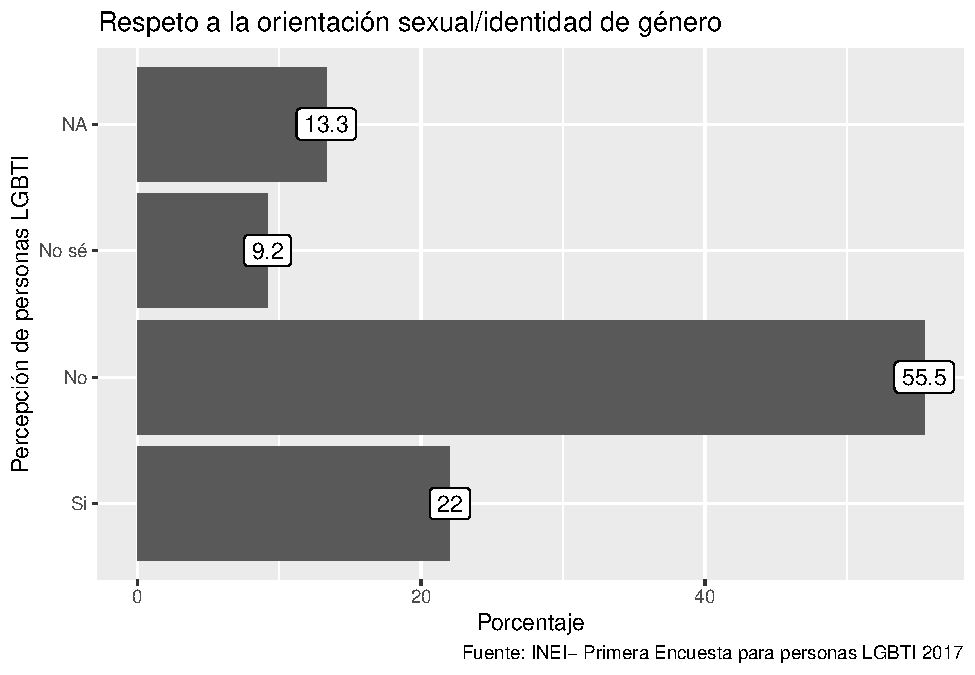
\includegraphics{02-LZM_files/figure-latex/unnamed-chunk-17-1.pdf}

De acuerdo al gráfico podemos identificar que del total de personas LGBTI encuestadas el \textbf{55.5\%} manifestó que la población peruana \textbf{no respeta su orientación sexual e identidad de género}; mientras que un 22\% indicó que sí siente ser respetada.

\begin{Shaded}
\begin{Highlighting}[]
\NormalTok{sociedad\_reconoce }\SpecialCharTok{\%\textgreater{}\%} 
  \FunctionTok{ggplot}\NormalTok{(}\FunctionTok{aes}\NormalTok{(porcentaje, p504)) }\SpecialCharTok{+}
  \FunctionTok{geom\_col}\NormalTok{() }\SpecialCharTok{+}
  \FunctionTok{geom\_label}\NormalTok{(}\FunctionTok{aes}\NormalTok{(}\AttributeTok{label =} \FunctionTok{round}\NormalTok{(porcentaje, }\DecValTok{1}\NormalTok{)))}\SpecialCharTok{+}
  \FunctionTok{labs}\NormalTok{(}\AttributeTok{title =} \StringTok{"Avance en el reconocimiento de los derechos humanos de las }\SpecialCharTok{\textbackslash{}n}\StringTok{ personas LGBTI en el Perú"}\NormalTok{, }
       \AttributeTok{caption =} \StringTok{"Fuente: INEI{-} Primera Encuesta para personas LGBTI 2017"}\NormalTok{) }\SpecialCharTok{+}
  \FunctionTok{labs}\NormalTok{(}\AttributeTok{x =} \StringTok{"Porcentaje"}\NormalTok{,}
       \AttributeTok{y =} \StringTok{"Percepción de personas LGBTI"}\NormalTok{)}
\end{Highlighting}
\end{Shaded}

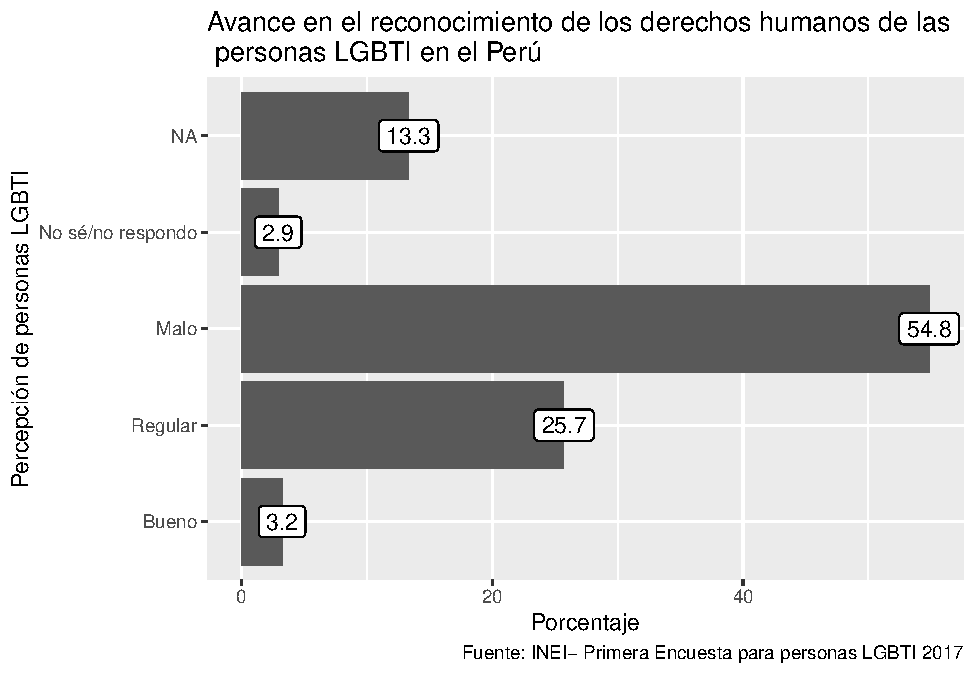
\includegraphics{02-LZM_files/figure-latex/unnamed-chunk-18-1.pdf}

Asimismo, de acuerdo a la información brindada por la población encuestada, la principal percepción en torno al avance del reconocimiento de los derechos humanos es negativa. Un 54.8\% considera que en Perú existe un mal avance, un 25.7\% que es regular y solo el 3.2\% considera que hay un buen avance.

En línea con lo anterior, a continuación ejecutamos un bloque de códigos que nos permite obtener un gráfico de barras a partir del cruce de las varibles \textbf{501} y \textbf{504}. Al respecto, la variable \textbf{501} se encuentra filtrada y presenta información en función a los valores Sí, No, No sé. Así, la información obtenida por la variable \textbf{504} se ordenará en estos tres grupos y de presentará la información porcentual por categorías ``No sé/ no respondo,'' ``Malo,'' ``Regular'' y ``Bueno.''

\begin{Shaded}
\begin{Highlighting}[]
\NormalTok{respeta\_reconoce }\SpecialCharTok{\%\textgreater{}\%} 
  \FunctionTok{ggplot}\NormalTok{(}\FunctionTok{aes}\NormalTok{(porcentaje, p504)) }\SpecialCharTok{+}
  \FunctionTok{geom\_col}\NormalTok{() }\SpecialCharTok{+}
  \FunctionTok{facet\_grid}\NormalTok{(}\AttributeTok{rows =} \StringTok{"p501"}\NormalTok{)}\SpecialCharTok{+}
  \FunctionTok{geom\_label}\NormalTok{(}\FunctionTok{aes}\NormalTok{(}\AttributeTok{label =} \FunctionTok{round}\NormalTok{(porcentaje, }\DecValTok{1}\NormalTok{)))}\SpecialCharTok{+}
  \FunctionTok{labs}\NormalTok{(}\AttributeTok{caption =} \StringTok{"Fuente: INEI{-} Primera Encuesta para personas LGBTI 2017"}\NormalTok{) }\SpecialCharTok{+}
  \FunctionTok{labs}\NormalTok{(}\AttributeTok{x =} \StringTok{"Porcentaje"}\NormalTok{,}
       \AttributeTok{y =} \StringTok{"Recocimiento de derechos humanos en personas LGBTI"}\NormalTok{)}
\end{Highlighting}
\end{Shaded}

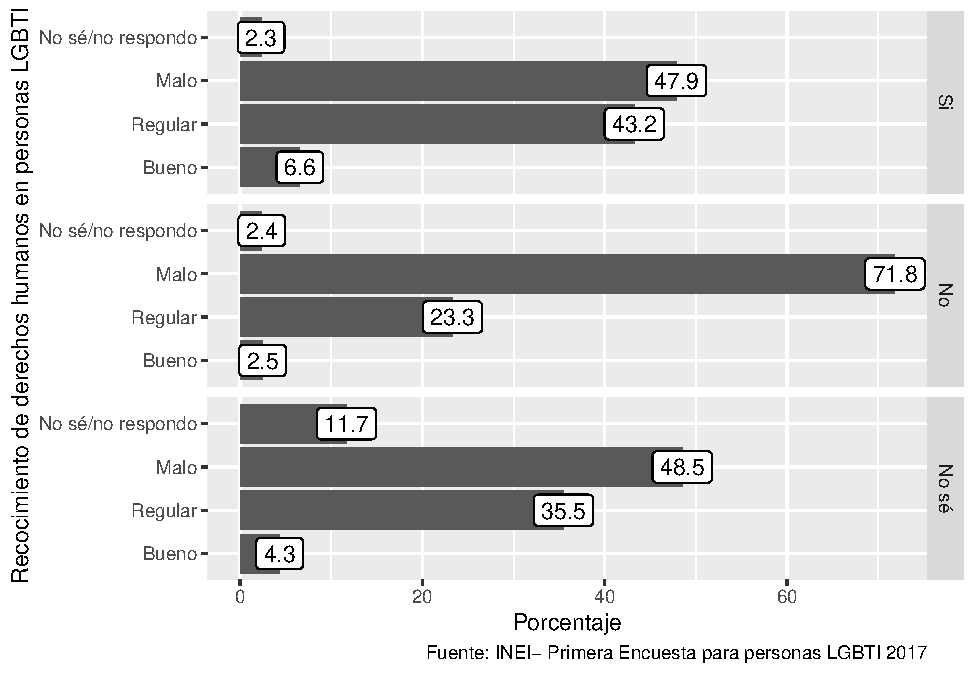
\includegraphics{02-LZM_files/figure-latex/unnamed-chunk-19-1.pdf}

En función al gráfico, podemos observar que del total de personas encuestadas, el mayor porcentaje se ubica en el bloque ``No'' con un 71.8\%. Es decir que el grupo que indicó que la sociedad \textbf{no respeta} su orientación sexual e identidad de género también afirma, en un \textbf{71.8\%}, que el avance del reconocimiento de los derechos humanos es malo. Asimismo, del total de personas que indicaron que la sociedad peruana \textbf{si respeta su orientación sexual e identidad de género el 47.9\% también manifestó un mal avance en el país}.

De acuerdo al Informe de la II Encuesta Nacional de Derechos Humanos, para el 2019, la población LGBTI que fue encuestada manifestó que el derecho que percibe como más vulnerado es el de un trato digno y no ser discriminación (51\%). De acuerdo a las estadísticas, el segundo derecho vulnerado sería la libertad de expresión y opinión (37\%). Asimismo, el informe indica que un grupo de la población peruana (45\%) considera que la homosexualidad es producto de algún trauma o que las personas trans viven confundidas.

\hypertarget{el-maltrato-gratuito-espacios-y-perpetradores-de-discriminaciuxf3n-yo-violencia.}{%
\subsection{El maltrato gratuito: Espacios y perpetradores de discriminación y/o violencia.}\label{el-maltrato-gratuito-espacios-y-perpetradores-de-discriminaciuxf3n-yo-violencia.}}

En relación con los resultados anteriores, resulta importante mencionar que en el Informe Defensorial N° 175, la Defensoría del Pueblo advertía que las personas LGBTI son víctimas de violencia y discriminación a razón de los estigmas, estereotios y prejuicios vinculados a su orientación sexual y/o identidad de género.

En ese sentido, cobra sustento que en el 2017, el 63\% de encuestadas que participaron de la Primera Encuesta Virtual para personas LGBTI hayan indicado haber sido víctimas de actos de discriminación y/o violencia.

El siguiente gráfico ayuda a identificar porcentualmente cuáles son los principales grupos etáreos que estarían comunicando el haber experimentado con mayor incidencia manifestaciones de discriminación y/o violencia.

\begin{Shaded}
\begin{Highlighting}[]
\NormalTok{grupo\_violencia }\SpecialCharTok{\%\textgreater{}\%} 
  \FunctionTok{ggplot}\NormalTok{(}\FunctionTok{aes}\NormalTok{(porcentaje, gedad)) }\SpecialCharTok{+}
  \FunctionTok{geom\_col}\NormalTok{()}\SpecialCharTok{+}
  \FunctionTok{geom\_label}\NormalTok{(}\FunctionTok{aes}\NormalTok{(}\AttributeTok{label =} \FunctionTok{round}\NormalTok{(porcentaje, }\DecValTok{1}\NormalTok{)))}\SpecialCharTok{+}
  \FunctionTok{labs}\NormalTok{(}\AttributeTok{title =} \StringTok{"Porcentaje de violencia recibida por grupos etáreos"}\NormalTok{, }
       \AttributeTok{caption =} \StringTok{"Fuente: INEI{-} Primera Encuesta para personas LGBTI 2017"}\NormalTok{) }\SpecialCharTok{+}
  \FunctionTok{labs}\NormalTok{(}\AttributeTok{x =} \StringTok{"Porcentaje"}\NormalTok{,}
       \AttributeTok{y =} \StringTok{"Grupos etáreos"}\NormalTok{)}
\end{Highlighting}
\end{Shaded}

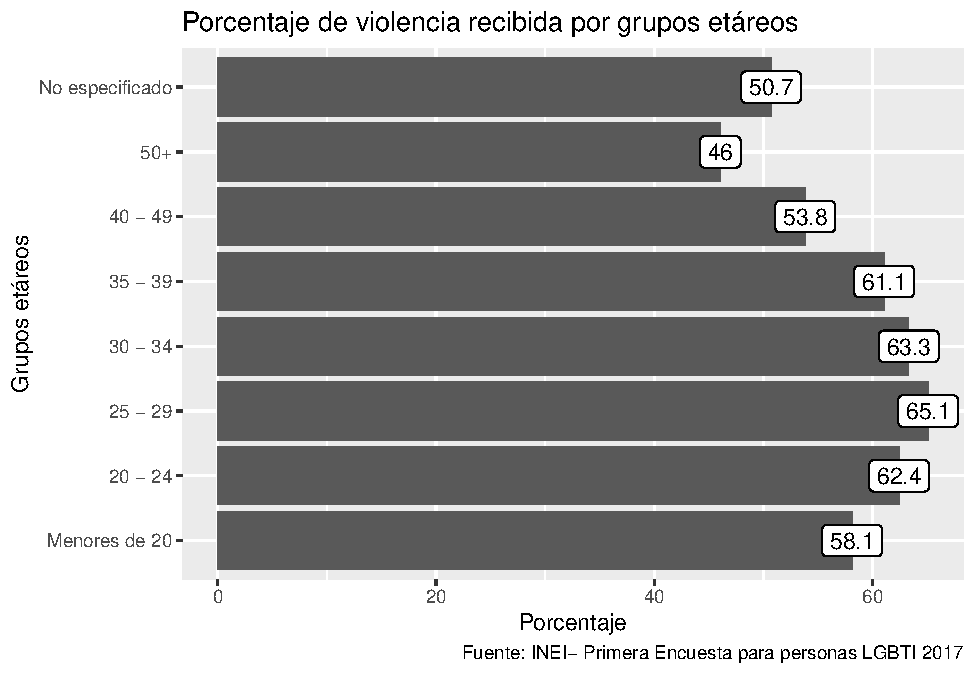
\includegraphics{02-LZM_files/figure-latex/unnamed-chunk-20-1.pdf}

Del gráfico, podemos identificar que existen cuatro grupos etáreos que registran mayores porcentajes respecto a haber sido víctima de discriminación y/o violencia. El primer grupo etáreo es del rango de 25 a 29 años con un 65.1\%, el segundo de 30 a 34 años con un 63.3\%, el tercer grupo es del rango de 20 a 24 años con un 62.4\% y el cuarto de 35 a 39 años con un 61.1\%.

Para el 2019, los resultados de la II Encuesta Nacional de Derechos Humanos arroja que en el Perú, una de las poblaciones que se percibe como más discriminada son las personas LGBTI. Del total de encuestados, la mayoría (47\%) indicó que las personas homosexuales, trans y bisexuales se encuentran en el grupo de \textbf{muy discriminados}. Junto con ello, se indica que para ese año la tercera razón (36\%) de discriminación en el Perú es la orientación sexual.

En línea con lo anterior, presentamos dos gráficos de barras con información relevante. El primero expone un gráfico de barras que presenta los principales ámbitos en donde las personas LGBTI han experimentado manifestaciones de discriminación y violencia; mientras que el segundo identifica, según lo manifestado por las personas encuestadas, los principales perpetradores de discriminación y/O violencia.

\begin{Shaded}
\begin{Highlighting}[]
\NormalTok{espacios\_violencia }\SpecialCharTok{\%\textgreater{}\%} 
  \FunctionTok{ggplot}\NormalTok{(}\FunctionTok{aes}\NormalTok{(porcentaje, name)) }\SpecialCharTok{+}
  \FunctionTok{geom\_col}\NormalTok{()}\SpecialCharTok{+}
  \FunctionTok{geom\_label}\NormalTok{(}\FunctionTok{aes}\NormalTok{(}\AttributeTok{label =} \FunctionTok{round}\NormalTok{(porcentaje, }\DecValTok{1}\NormalTok{)))}\SpecialCharTok{+}
    \FunctionTok{labs}\NormalTok{(}\AttributeTok{title =} \StringTok{"Principales espacios de violencia"}\NormalTok{, }
       \AttributeTok{caption =} \StringTok{"Fuente: INEI{-} Primera Encuesta para personas LGBTI 2017"}\NormalTok{) }\SpecialCharTok{+}
  \FunctionTok{labs}\NormalTok{(}\AttributeTok{x =} \StringTok{"Porcentaje"}\NormalTok{,}
       \AttributeTok{y =} \StringTok{"Espacios/Lugares"}\NormalTok{)}
\end{Highlighting}
\end{Shaded}

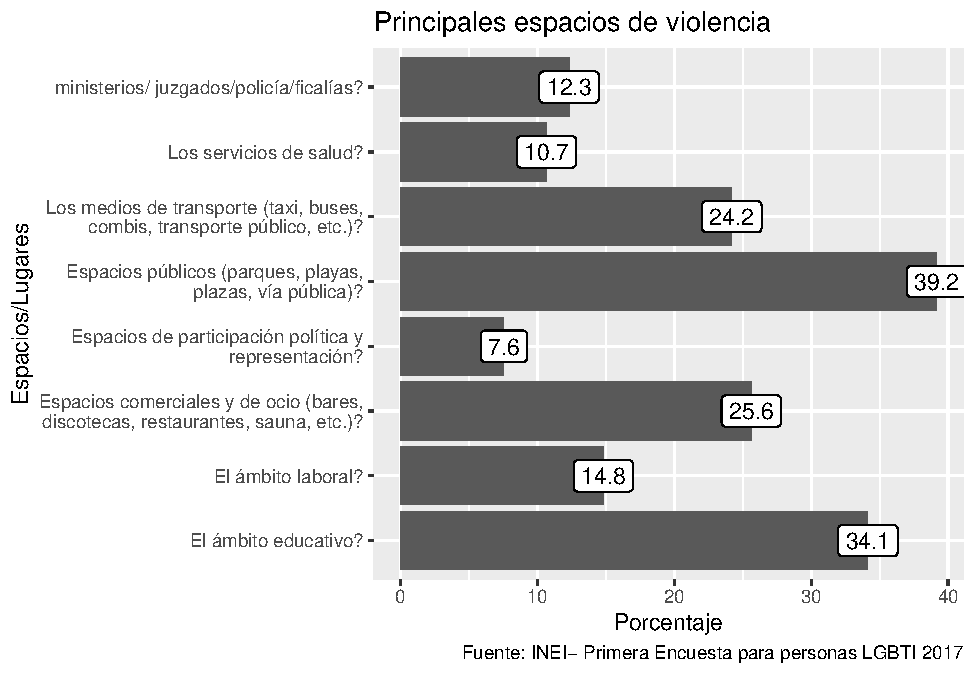
\includegraphics{02-LZM_files/figure-latex/unnamed-chunk-21-1.pdf}

De la información brindada, podemos observar que los espacios públicos como parques, playas, plazas y vía pública son identificados en un 39.2\% como el principal ámbito en donde las personas LGBTI experimentaron ser víctimas de alguna muestra de discriminación y/o violencia. El segundo ámbito identificado es el educativo con un 34.1\%.

Si consideramos que actualmente no se cuenta con una segunda encuesta virtual para personas LGBTI u otro instrumento específico para esta población que permita recabar información estadística desde el Estado, los resultados presentados durante el 2017 son preocupantes porque evidencian que los espacios públicos son asimilados como ámbitos inseguros para personas LGBTI, en donde existe una potencial vulneración al derecho a un trato digno y libertad de expresión y opinión.

Para autoras como Fraser, la instalación de una esfera pública homogénea aisla los espacios discursivos, cierra la puertas al debate e imposibilita la igualdad de participación debido a un marco institucional que crea grupos sociales dominanres y subordinados (1997, pag 95-133)

\begin{Shaded}
\begin{Highlighting}[]
\NormalTok{ejercen\_violencia }\SpecialCharTok{\%\textgreater{}\%} 
  \FunctionTok{ggplot}\NormalTok{(}\FunctionTok{aes}\NormalTok{(porcentaje, name)) }\SpecialCharTok{+}
  \FunctionTok{geom\_col}\NormalTok{()}\SpecialCharTok{+}
  \FunctionTok{geom\_label}\NormalTok{(}\FunctionTok{aes}\NormalTok{(}\AttributeTok{label =} \FunctionTok{round}\NormalTok{(porcentaje, }\DecValTok{1}\NormalTok{)))}\SpecialCharTok{+}
    \FunctionTok{labs}\NormalTok{(}\AttributeTok{title =} \StringTok{"Principales perpetradores de violencia hacia }\SpecialCharTok{\textbackslash{}n}\StringTok{ personas LGBTI"}\NormalTok{, }
       \AttributeTok{caption =} \StringTok{"Fuente: INEI{-} Primera Encuesta para personas LGBTI 2017"}\NormalTok{) }\SpecialCharTok{+}
  \FunctionTok{labs}\NormalTok{(}\AttributeTok{x =} \StringTok{"Porcentaje"}\NormalTok{,}
       \AttributeTok{y =} \StringTok{"Personas / Perfiles"}\NormalTok{)}
\end{Highlighting}
\end{Shaded}

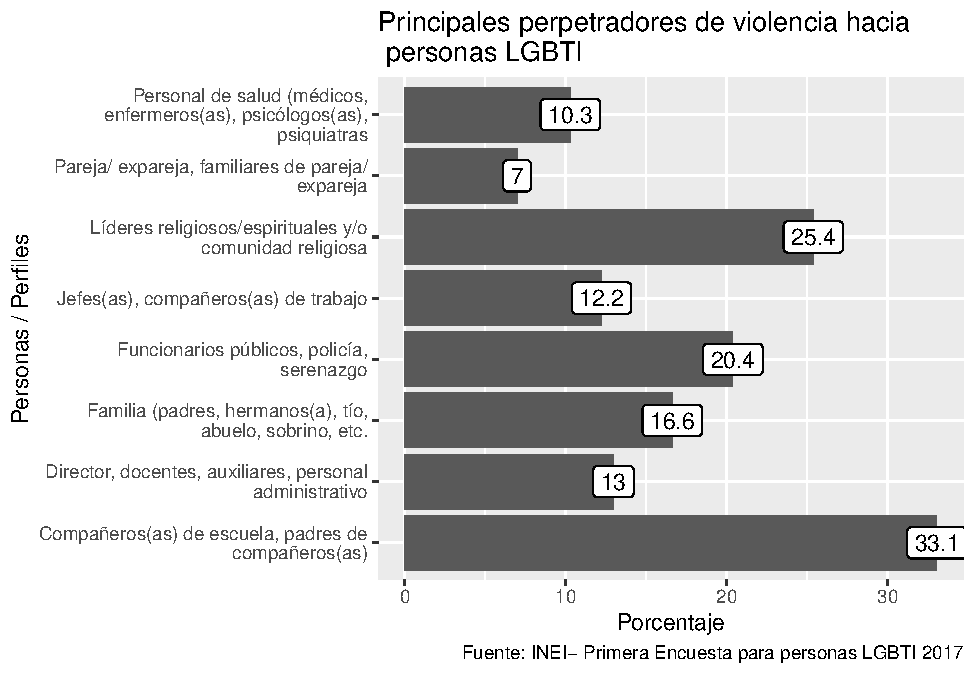
\includegraphics{02-LZM_files/figure-latex/unnamed-chunk-22-1.pdf}
Asimismo, considerando que los resultados posicionan como los principales perpetradores de discriminaicón y/o violancia hacia las personas LGBTI a compañeros(as) de escuela y padres de compañeros(as) con 33.1\%, preocupa las consecuencias que estaría generando la violencia homofóbica o transfóbica en el ámbito educativo.

De acuerdo a la Defensoría del Pueblo (2015), este tipo de violencia genera en los estudiantes dificultades para prestar atención en clases, empeorar calificaciones, abandonar o cambiar de institución.

Junto con ello, también resulta importante leer estos resultados en su relación con la construcción de la ciudadanía y la democracia. A saber, según estudios que analizan ambos temas, las familias esperan que la democracia y la escuela ayuden a construir mejores condiciones de vida y oportunidades. En esa línea, el ámbito educativo es crucial para mejorar la relación entre ciudadanos, Estado y demoracia si el sistema educativo brinda un servicio de calidad para todos y todas (2015, pág 6)

\hypertarget{participaciuxf3n-ciudadana-vinculaciuxf3n-con-organizaciones-y-principales-acciones.}{%
\subsection{Participación ¿ciudadana?: Vinculación con organizaciones y principales acciones.}\label{participaciuxf3n-ciudadana-vinculaciuxf3n-con-organizaciones-y-principales-acciones.}}

Al igual que el término democracia, el termino participación ciudadana ha sido empleado de manera diversa, en contextos y propósitos diferenciados. Para autores como Serrano, resulta importante diferenciar la participación ciudadana y la participación política ciudadana; para él (2009), tomando como referencia a Cunill, la participación ciudadana está orientada a promover y crear nuevos mecanismos para que la administración conozca mejor las actividades de sus administrados; en ese sentido, se pueda generar una colaboración conjunta para la ejecución de algunas tareas o se sustituya al Estado en la relación de determinadas funciones.

En esa línea, considera que la participación ciudadana puede ser comprendida como una herramienta importante que ayuda a advertir la necesidad de optimizar los procedimientos institucionales frente a la pérdida de eficacia de sus mecanismos tradicionales. Así, la participación ciudadana puede ser ubicada como herramienta para la gestión.

Diferente a ello, menciona que la participación política ciudadana se ejerce cuando existe un interés de tipo político; es decir, ``la búsqueda de la trascendencia e incidencia de las opiniones de los particulares en la toma de decisiones de interéses públicos que de manera tradicional están en manos de partidos políticos y grupos de poder''

Para fines del presente proyecto, nos resulta interesante tomar la propuesta de Velásquez (2010), quien habla de la participación como proceso que no se restringue a lo institucional-normativo. Para él, la participaicón ciudadana ``es el proceso mdiante el cual diferntes actores (sociales, económicos, políticos), en forma individual o colectiva y en función de sus necesidades, intereses, recursos y motivaciones, intervienen en el escenario públilco con el fin de obtener bienes y sercicios públicos y/o de incidir en la definición de ausntos de interpes colectivo''

Así, diferencia este tipo de participación de la político-electoral, oarticipaicón social o comunitaria Para él se trata de la incidencia en la formulación, ejecución y seguimiento de las políticas públicas.

En tal sentido, es relevante indicar que, en función a la revisión de la data y la manera en cómo se encuentran configuradas las preguntas sobre participación ciudadana, no se cuenta con información suficiente que ayude a comprender la repercusión o incidencia que las personas LGBTI estarían generando en el marco del ciclo de las políticas públicas. A diferencia de ello, solo sería posible identificar la vinculación que tienen con determinados tipos de organizaciones y las principales acciones que desarrollan.

En ese sentido, a continuación se presenta un gráfico con la distribución porcentual de los principales tipos de organización a los que estarían adcritas o con las que mantendrían vinculación las personas LGBTI.

\begin{Shaded}
\begin{Highlighting}[]
\NormalTok{organizaciones }\SpecialCharTok{\%\textgreater{}\%} 
  \FunctionTok{ggplot}\NormalTok{(}\FunctionTok{aes}\NormalTok{(porcentaje, name)) }\SpecialCharTok{+}
  \FunctionTok{geom\_col}\NormalTok{()}\SpecialCharTok{+}
  \FunctionTok{geom\_label}\NormalTok{(}\FunctionTok{aes}\NormalTok{(}\AttributeTok{label =} \FunctionTok{round}\NormalTok{(porcentaje, }\DecValTok{1}\NormalTok{)))}\SpecialCharTok{+}
    \FunctionTok{labs}\NormalTok{(}\AttributeTok{title =} \StringTok{"Vinculación de personas LGBTI en organizaciones"}\NormalTok{, }
       \AttributeTok{caption =} \StringTok{"Fuente: INEI{-} Primera Encuesta para personas LGBTI 2017"}\NormalTok{) }\SpecialCharTok{+}
  \FunctionTok{labs}\NormalTok{(}\AttributeTok{x =} \StringTok{"Porcentaje"}\NormalTok{,}
       \AttributeTok{y =} \StringTok{"Tipo de organizaciones"}\NormalTok{)}
\end{Highlighting}
\end{Shaded}

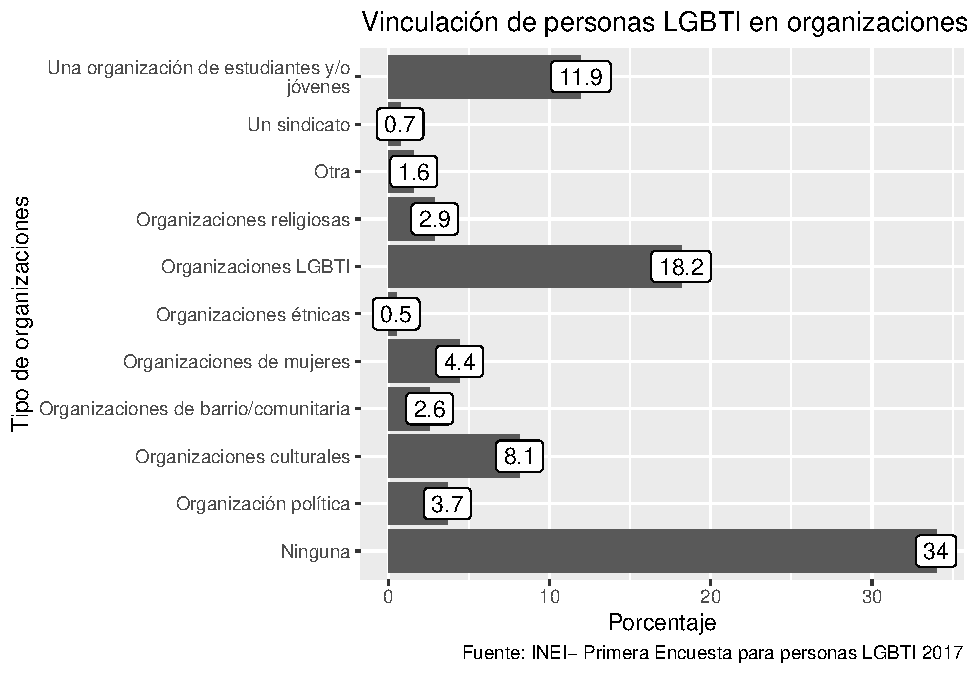
\includegraphics{02-LZM_files/figure-latex/unnamed-chunk-23-1.pdf}

El gráfico nos muestra que del total de las personas encuestadas la mayoría (34\%) no tiene ninguna vinculación con organizaciones. También indica que el segundo bloque mayoritario manifiesta que está vinculado con organizaciones LGBTI (18.2\%) y que entre los menores porcentajes se encuentra la participación en organizaciones políticas (3.7\%)

En relación a la vinculación con alguna organización o no, el gráfico que se muestra a continuación muestra las principales acciones en las que participan los miembros de la comunidad LGBTI.

\begin{Shaded}
\begin{Highlighting}[]
\NormalTok{acciones\_organizaciones }\SpecialCharTok{\%\textgreater{}\%} 
  \FunctionTok{ggplot}\NormalTok{(}\FunctionTok{aes}\NormalTok{(porcentaje, acciones)) }\SpecialCharTok{+}
  \FunctionTok{geom\_col}\NormalTok{() }\SpecialCharTok{+}
  \FunctionTok{facet\_wrap}\NormalTok{(}\SpecialCharTok{\textasciitilde{}}\NormalTok{tipo\_organizacion, }\AttributeTok{nrow =} \DecValTok{4}\NormalTok{)}\SpecialCharTok{+}
  \FunctionTok{geom\_label}\NormalTok{(}\FunctionTok{aes}\NormalTok{(}\AttributeTok{label =} \FunctionTok{round}\NormalTok{(porcentaje, }\DecValTok{1}\NormalTok{)))}\SpecialCharTok{+}
  \FunctionTok{labs}\NormalTok{(}\AttributeTok{caption =} \StringTok{"Fuente: INEI{-} Primera Encuesta para personas LGBTI 2017"}\NormalTok{) }\SpecialCharTok{+}
  \FunctionTok{labs}\NormalTok{(}\AttributeTok{x =} \StringTok{"Porcentaje"}\NormalTok{,}
       \AttributeTok{y =} \StringTok{"Acciones"}\NormalTok{)}
\end{Highlighting}
\end{Shaded}

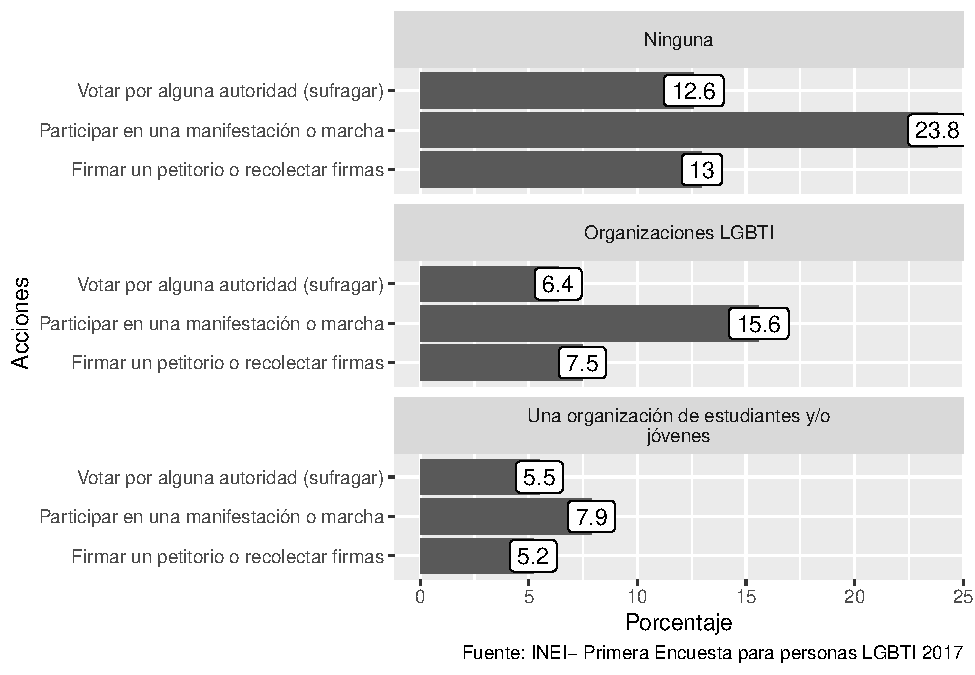
\includegraphics{02-LZM_files/figure-latex/unnamed-chunk-24-1.pdf}

Según lo registrado, podemos observar que si bien la mayoría de personas encuestadas manifestó no pertenecer a ninguna organización no se encuentran ajenas a desarrollar acciones vinculadas a participación ciudadana. Así lo manifestó el 23.8\% que indicó haber participado en una manifestación o marcha. Esta acción también es la que predomina en las personas que indicaron pertenecer a organizaciones LGBTI o de estudiantes y/o jóvenes.

Para fines de la investigación, nos parece relevante los resultados obtenidos en el siguiente gráfico. De acuerdo a la información, no existen cambios porcentuales respecto a la participación o vinculación a una organización en personas que indicaron haber sido víctimas de discriminación y violencia. Al respecto, también observamos que del total de personas la mayoría no se encuentra vinculada con ninguna organización (41\%);asimismo, el segundo grupo mayoritario también indica pertenecer a organizaciones LGBTI (24\%), seguido de un 14.7 que mantiene vinculación con organizacones de estudiantes y/o jóvenes. Entre los menores porcentajes también se ubican las organizaciones políticas (4.4\%).

\begin{Shaded}
\begin{Highlighting}[]
\NormalTok{personasviol\_organizaciones }\SpecialCharTok{\%\textgreater{}\%} 
  \FunctionTok{ggplot}\NormalTok{(}\FunctionTok{aes}\NormalTok{(porcentaje, tipo\_organizacion)) }\SpecialCharTok{+}
  \FunctionTok{geom\_col}\NormalTok{()}\SpecialCharTok{+}
  \FunctionTok{geom\_label}\NormalTok{(}\FunctionTok{aes}\NormalTok{(}\AttributeTok{label =} \FunctionTok{round}\NormalTok{(porcentaje, }\DecValTok{1}\NormalTok{)))}\SpecialCharTok{+}
    \FunctionTok{labs}\NormalTok{(}\AttributeTok{title =} \StringTok{"Participación por tipo de organizaciones de personas }\SpecialCharTok{\textbackslash{}n}\StringTok{ LGBTI violentadas o discriminadas"}\NormalTok{, }
       \AttributeTok{caption =} \StringTok{"Fuente: INEI{-} Primera Encuesta para personas LGBTI 2017"}\NormalTok{) }\SpecialCharTok{+}
  \FunctionTok{labs}\NormalTok{(}\AttributeTok{x =} \StringTok{"Porcentaje"}\NormalTok{,}
       \AttributeTok{y =} \StringTok{"Tipo de organizaciones"}\NormalTok{)}
\end{Highlighting}
\end{Shaded}

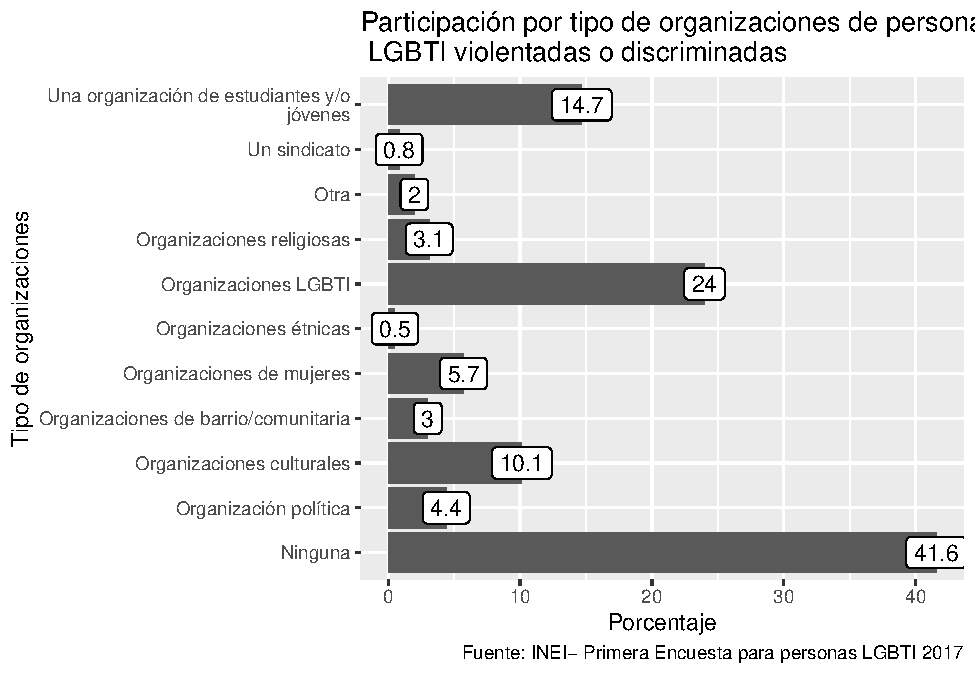
\includegraphics{02-LZM_files/figure-latex/unnamed-chunk-25-1.pdf}

Ahora bien, respecto a las acciones de participación ciudadana desarrolladas por personas que experimentaron discriminación y/o violencia, identificamos que la mayoría opta por participar en una manifstación o marcha (53.3\%); a este porcentaje le sigue un 33.3 que afirma haber desarrollado acciones vinculadas a votar por alguna autoridad. El menor porcentaje lo registra postular a cargos públicos con un 1.4\%.

\begin{Shaded}
\begin{Highlighting}[]
\NormalTok{personasviol\_acciones }\SpecialCharTok{\%\textgreater{}\%} 
  \FunctionTok{ggplot}\NormalTok{(}\FunctionTok{aes}\NormalTok{(porcentaje, acciones)) }\SpecialCharTok{+}
  \FunctionTok{geom\_col}\NormalTok{()}\SpecialCharTok{+}
  \FunctionTok{geom\_label}\NormalTok{(}\FunctionTok{aes}\NormalTok{(}\AttributeTok{label =} \FunctionTok{round}\NormalTok{(porcentaje, }\DecValTok{1}\NormalTok{)))}\SpecialCharTok{+}
    \FunctionTok{labs}\NormalTok{(}\AttributeTok{title =} \StringTok{"Acciones desarrolladas por personas LGBTI violentadas }\SpecialCharTok{\textbackslash{}n}\StringTok{ o discriminadas"}\NormalTok{, }
       \AttributeTok{caption =} \StringTok{"Fuente: INEI{-} Primera Encuesta para personas LGBTI 2017"}\NormalTok{) }\SpecialCharTok{+}
  \FunctionTok{labs}\NormalTok{(}\AttributeTok{x =} \StringTok{"Porcentaje"}\NormalTok{,}
       \AttributeTok{y =} \StringTok{"acciones"}\NormalTok{)}
\end{Highlighting}
\end{Shaded}

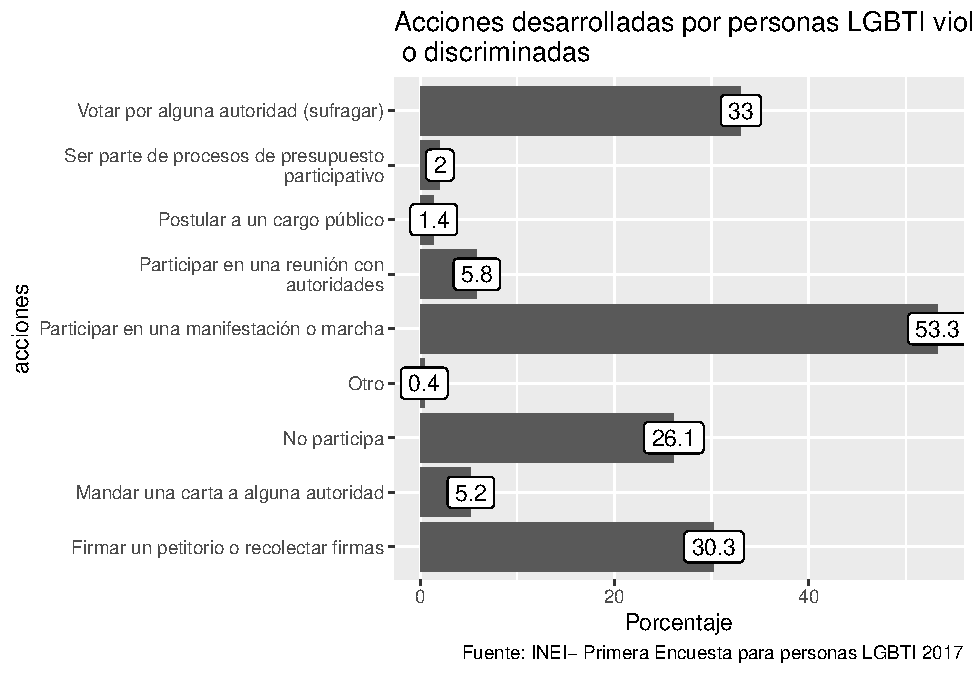
\includegraphics{02-LZM_files/figure-latex/unnamed-chunk-26-1.pdf}

A partir de los resultados obtenidos, quisimos observar el nivel educativo al que pertenecen los encuestados por acciones. Para ello, calculamos en primer lugar la distribución de la muestra. Al respecto, ésta presenta como categorías con mayor porcentaje a \textbf{superior universitaria Incompleta con 29.3\%} y \textbf{superior universitaria completa con 27.6\%}, de acuerdo al siguiente gráfico.

\begin{Shaded}
\begin{Highlighting}[]
\NormalTok{recuento\_niveledu }\SpecialCharTok{\%\textgreater{}\%} 
  \FunctionTok{ggplot}\NormalTok{(}\FunctionTok{aes}\NormalTok{(porcentaje, p101)) }\SpecialCharTok{+}
  \FunctionTok{geom\_col}\NormalTok{() }\SpecialCharTok{+}
  \FunctionTok{geom\_label}\NormalTok{(}\FunctionTok{aes}\NormalTok{(}\AttributeTok{label =} \FunctionTok{round}\NormalTok{(porcentaje, }\DecValTok{1}\NormalTok{)))}\SpecialCharTok{+}
  \FunctionTok{labs}\NormalTok{(}\AttributeTok{title =} \StringTok{"Distribución del nivel educativo en la muestra"}\NormalTok{, }
       \AttributeTok{caption =} \StringTok{"Fuente: INEI{-} Primera Encuesta para personas LGBTI 2017"}\NormalTok{) }\SpecialCharTok{+}
  \FunctionTok{labs}\NormalTok{(}\AttributeTok{x =} \StringTok{"Porcentaje"}\NormalTok{,}
       \AttributeTok{y =} \StringTok{"Nivel educativo"}\NormalTok{)}
\end{Highlighting}
\end{Shaded}

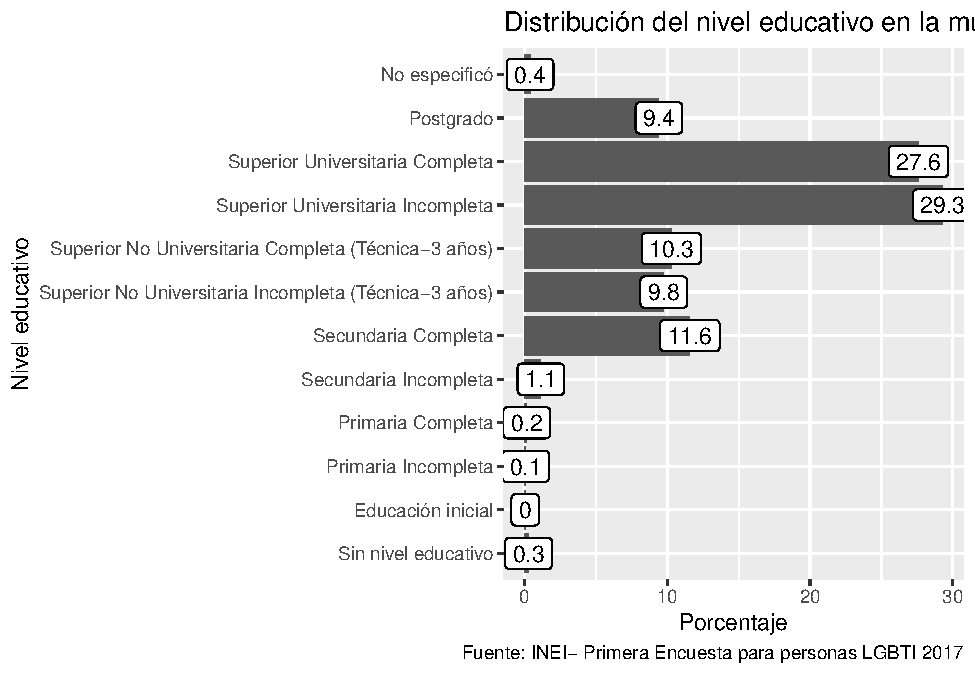
\includegraphics{02-LZM_files/figure-latex/unnamed-chunk-27-1.pdf}

En línea con el gráfico anterior, observamos que los resultados que arroja el siguiente podrían ser reflejo de los anteriores. En ese sentido, no permite ver que la categoría nivel educativo determine el desarrollo de las acciones participativas.

\begin{Shaded}
\begin{Highlighting}[]
\NormalTok{niveleduc\_participacion }\SpecialCharTok{\%\textgreater{}\%} 
  \FunctionTok{ggplot}\NormalTok{(}\FunctionTok{aes}\NormalTok{(porcentaje, acciones)) }\SpecialCharTok{+}
  \FunctionTok{geom\_col}\NormalTok{(}\FunctionTok{aes}\NormalTok{(}\AttributeTok{fill =}\NormalTok{ p101)) }\SpecialCharTok{+}
  \FunctionTok{geom\_label}\NormalTok{(}\FunctionTok{aes}\NormalTok{(}\AttributeTok{label =} \FunctionTok{round}\NormalTok{(porcentaje, }\DecValTok{1}\NormalTok{)), }\AttributeTok{position =} \FunctionTok{position\_stack}\NormalTok{())}\SpecialCharTok{+}
  \FunctionTok{labs}\NormalTok{(}\AttributeTok{caption =} \StringTok{"Fuente: INEI{-} Primera Encuesta para personas LGBTI 2017"}\NormalTok{) }\SpecialCharTok{+}
  \FunctionTok{labs}\NormalTok{(}\AttributeTok{x =} \StringTok{"Porcentaje"}\NormalTok{,}
       \AttributeTok{y =} \StringTok{"p101"}\NormalTok{)}
\end{Highlighting}
\end{Shaded}

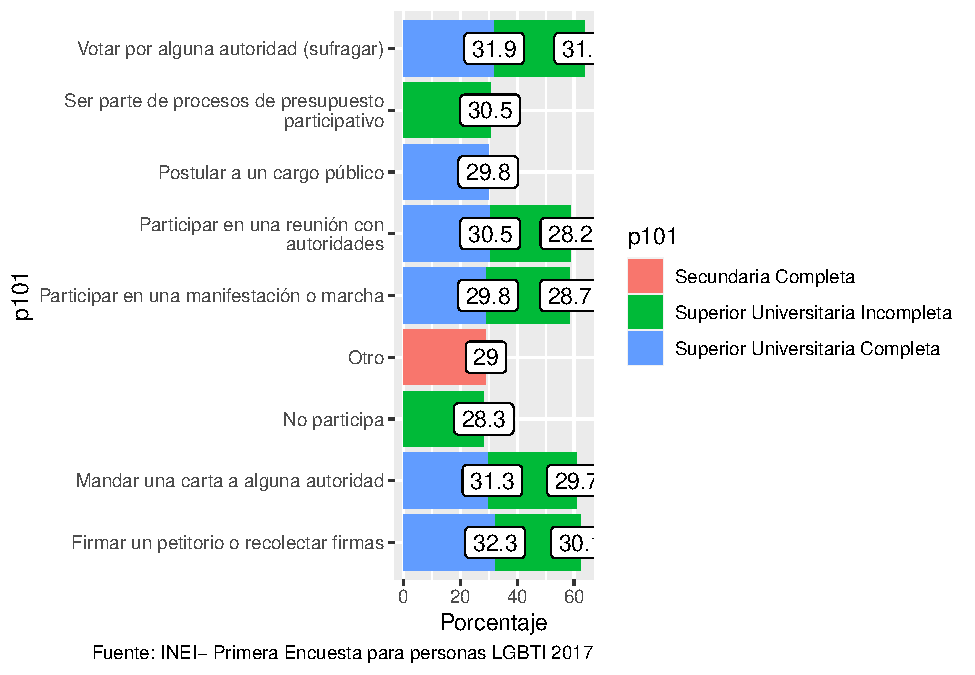
\includegraphics{02-LZM_files/figure-latex/unnamed-chunk-28-1.pdf}

A continuación observamos que del total de la población que manifestó experimentar alguna muestra de discrimininación y/o violencia, el mayor porcentaje de respuestas (64.7\%) se ubica en el bloque de personas que indicaron \textbf{no expresar librevemete su orientación sexual o identidad de género} precisando que \textbf{no participa de ninguna acción}.El segundo porcentaje mayoritario también se ubica en el mismo bloque indicando *ser parte de procesos de presupuesto participativo\textbf{ (61.5\%). Respecto al bloque que indicó }expresar librevemte su orientación sexual o identidad de género\textbf{ el 50.8\% manifestó que }participó en reuniones con autoridades\textbf{, seguido de un 45.5\% que señaló haber }mandado una carta a alguna autoridad**

\begin{Shaded}
\begin{Highlighting}[]
\NormalTok{expresion\_participa }\SpecialCharTok{\%\textgreater{}\%}
  \FunctionTok{ggplot}\NormalTok{(}\FunctionTok{aes}\NormalTok{(porcentaje, acciones)) }\SpecialCharTok{+}
  \FunctionTok{geom\_col}\NormalTok{(}\FunctionTok{aes}\NormalTok{(}\AttributeTok{fill =}\NormalTok{ p116), }\AttributeTok{position =} \FunctionTok{position\_dodge}\NormalTok{(}\DecValTok{1}\NormalTok{)) }\SpecialCharTok{+}
  \FunctionTok{geom\_label}\NormalTok{(}\FunctionTok{aes}\NormalTok{(}\AttributeTok{label =} \FunctionTok{round}\NormalTok{(porcentaje, }\DecValTok{1}\NormalTok{), }\AttributeTok{group =}\NormalTok{ p116), }
             \AttributeTok{position =} \FunctionTok{position\_dodge}\NormalTok{(}\DecValTok{1}\NormalTok{), }\AttributeTok{size =} \FloatTok{2.5}\NormalTok{)}\SpecialCharTok{+}
  \FunctionTok{labs}\NormalTok{(}\AttributeTok{caption =} \StringTok{"Fuente: INEI{-} Primera Encuesta para personas LGBTI 2017"}\NormalTok{) }\SpecialCharTok{+}
  \FunctionTok{labs}\NormalTok{(}\AttributeTok{x =} \StringTok{"Porcentaje"}\NormalTok{,}
       \AttributeTok{y =} \StringTok{"acciones"}\NormalTok{,}
       \AttributeTok{fill =} \StringTok{"Expresa libremente"}
\NormalTok{       )}
\end{Highlighting}
\end{Shaded}

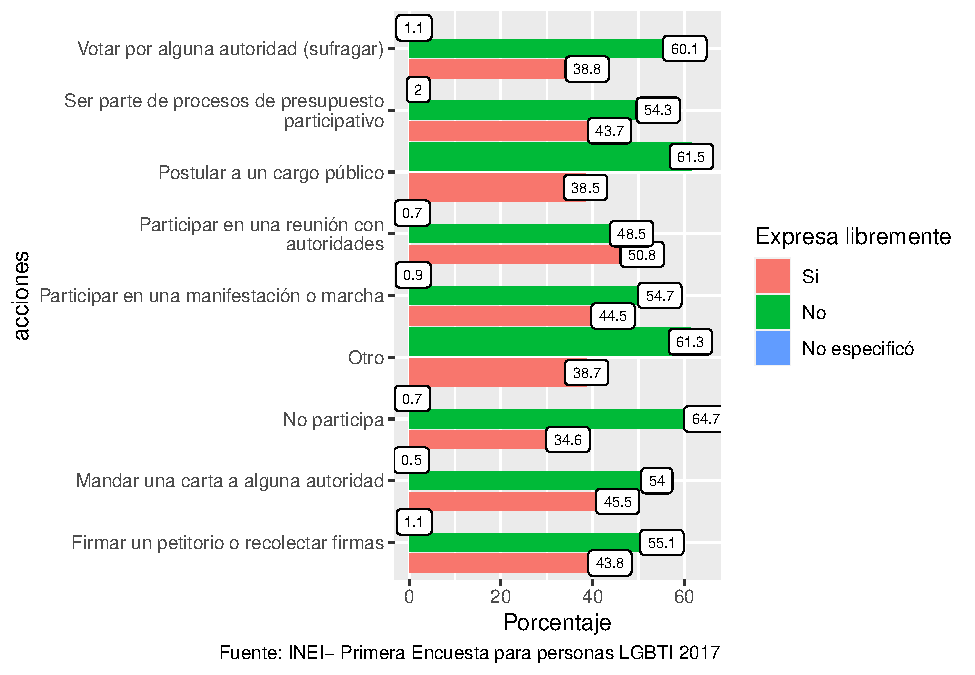
\includegraphics{02-LZM_files/figure-latex/unnamed-chunk-29-1.pdf}

\hypertarget{conclusiones}{%
\section{Conclusiones}\label{conclusiones}}

La exploración de variables vinculadas a percepción dan cuenta que existe un escenario desfavorable en torno al respeto hacia la orientación sexual e identidad de género de las personas LGBTQ+, así como el avance en el reconocimiento de sus derechos humanos.

De acuerdo a los porcentajes obtenidos se concluye que las personas que indicaron que la sociedad no respeta su orientación sexual e identidad de género manifiestan como respuesta frecuente (71.8\%) que el avance en el reconocimiento de los derechos humanos es malo. La misma afirmación fue identificada como respuesta frecuente (47.9\%) por quienes indicaron que la sociedad sí respeta su orientación sexual e identidad de género.

Si bien el INEI no ha desarrollado la Segunda Encuesta Virtual para personas LGBTI u otra encuesta orientada específicamente a obtener información sobre este grupo poblacional, se cuenta con información estadística generada por otros entidades o instituciones que guardar coherencia con la obtenida en la Primera Encuesta Virtual para personas LGBTI. Por ejemplo, la II Encuesta de Derechos Humanos indica que para el 2019 la población LGBTI que fue encuestada manifestó que el derecho que percibe como más vulnerado es el de un trato digno y no ser discriminación (51\%).

El escenario desfavorable en torno al respecto a la orientación sexual e identidad de género de las personas LGBTQ+ y los ínfimos avances que se tienen en materia de reconocimiento de derechos humanos perpetúan acciones y comportamientos de discriminación y/o violencia en espacios públicos y educativos. Esto podría estar limitando la participaicón en la esfera pública de las personas LGBTI si consideramos que del total de encuestados que manifestó experimentar alguna muestra de discrimininación y/o violencia, el mayor porcentaje (64.7\%) se ubicó en el bloque no expresar librevemente su orientación sexual o identidad de género precisando que no participa de ninguna acción.

Los resultados obtenidos permiten afirmar que para comprender la participación ciudadana de las personas LGBTQ+, en los términos que este proyecto propone, se requiere del desarrollo y aplicación de mecanismos permanentes e idóneos que generen información estadística confiable y actualizada sobre la situación de los derechos humanos de este grupo poblacional, en realación a ámbitos como educación, salud, integridad, comportamiento electoral y otros.

Al respecto, resulta importante indicar que para el ciudadano, el Estado representa una organización, una posibilidad, una acción y un responsable respecto a la provisión de diferentes bienes y servicios que deberían cubrir necesidades insatisfechas que atienden expectativas de calidad de vida (Ausejo, 2008). Sin embargo, en momentos donde se cuestiona el accionar de las autoridades y la legitimidad de las instituciones, por la carencia de atención o insuficientes mecanismos que hagan visibles las diferencias, tenderíamos a pensar que es resposabilidad del ciudadano comprender y participar de procesos que inciden en la calidad de vida de la colectividad.

Pero ¿qué ocurre si los espacios públicos en donde debería ser factible manifestar las demandas representan escenarios de inseguridad, discriminación y violencia?. Asimismo, ¿cómo esperamos que las personas LGBTI desarrollen y ejerza una participación ciudadana no condicionada si los espacios educativos violentan y estigmatizan aquello que está fuera del esquema heteronormativo?

Finalmente, esta aproximación permite identificar limitaciones y abrir otras preguntas de investigación que son necesarias para pensar la configuración de la participación ciudadana en las personas LGBTQ+.

\hypertarget{referencias}{%
\section{Referencias}\label{referencias}}

Ausejo (2008) De las Políticas Públicas a la gestión pública: una visión sistémica. Pease, G.; Villafranca, L.(Ed) El papel de las políticas públicas (29-36) Recuperado de: \url{https://escuela.pucp.edu.pe/gobierno/images/documentos/publicaciones/reforma2009.pdf}

Cunill, N. (1997) Repensando lo público a través de la sociedad. Nuevas formas de gestión pública y representación social, Venezuela, Nueva Sociedad. Recuperado de: \url{http://sitp.pichincha.gob.ec/repositorio/diseno_paginas/archivos/Repensando\%20lo\%20p\%C3\%BAblico\%20a\%20trav\%C3\%A9s\%20de\%20la\%20sociedad.pdf}

Dahl, R. (1989) La Poliarquía. Participaicón y oposición, Madrid: Editorial Tecnos (Grupo Anaya, S.A)

Defensoría del Pueblo (2016) Informe Defensorial N° 175 ``Derechos humanos de las personas LGBTI: Necesidades de una política pública para la igualdad en el Perú.'' Recuperado de: \url{https://www.defensoria.gob.pe/wp-content/uploads/2018/05/Informe-175--Derechos-humanos-de-personas-LGBTI.pdf}

Defensoría del Pueblo (2018) Informe de Adjuntía N° 007-2018-DP/ADHPD. ``A dos años del Informe Defensorial N° 175''Derechos humanos de las personas LGBTI: Necesidades de una política pública para la igualdad en el Perú". Recuperado de: \url{https://www.defensoria.gob.pe/wp-content/uploads/2018/12/Informe-Defensorial-N\%C2\%B0-007-2018-DPADHPD-\%E2\%80\%9CA-2-a\%C3\%B1os-del-Informe-Defensorial-N\%C2\%B0-175.-Estado-actual-de-los-derechos-de-las-personas-LGBTI\%E2\%80\%9D.pdf}

Fraser, N.(1997) Iustitia Interumpa: Reflexiones críticas desde la posición ``postsocialista.'' ``Pensando de nuevo la esfera pública.'' Santafé de Bogotá: Siglo del hombre editores. Facultad de Derecho, 1997.pp, 95-133.

Held, D. (2008) Modelos de Democracia, Madrid: Alianza Editorial.

Instituto de Estudios Peruanos (2016) La ciudadanía desde la escuela: democracia y ciudadanía. Recuperado de: \url{https://iep.org.pe/wp-content/uploads/2015/12/la_ciudadania_desde_la_escuela__democracia_y_ciudadania-1.pdf}

Instituto Nacional de Estadística e Informática (2018) Primera Encuesta Virtual para Personas LGBTI. Principales Resultados. Recuperado de: \url{https://www.inei.gob.pe/media/MenuRecursivo/boletines/lgbti.pdf}

López, J.;López, J. (2009) La participaicón política ciudadana; sus límites y controles institucionales en el caso mexicano. Estudios Políticos, vol.~9, num. 16, enero-abril, 2009, pp.~9-46. Universidad Nacional Autónoma de México. Recuperado en:\url{https://www.redalyc.org/pdf/4264/426439540001.pdf}

John, R. (2012) Participación ciudadana de la población LGBT en la localidad de Chapinero del 2007 al 2009, (tesis de maestría) Bogotá D.C-Colombia, Pontificia Universidad Javeriana, Maestría en Estudios Políticos. Recuperado de: \url{https://repository.javeriana.edu.co/bitstream/handle/10554/1389/RodriguezGarciaJohnMarlon2011.pdf;jsessionid=793E40824B1DD5FB7CCD6EE7288BA3AF?sequence=1}

Ministerio de Justicia y Derechos Humanos (2019) II Encuesta Nacional de Derechos Humanos. Informe Completo. Recuperado de: \url{https://cdn.www.gob.pe/uploads/document/file/1611180/3.-Informe-completo-de-la-II-Encuesta-Nacional-de-Derechos-Humanos.pdf.pdf}

Restrepo, J. (2005) Estándares Básicos en Competencias Ciudadanas: ¿Cuál concepción ciudadana?: Una aproximación teórica al problema de la formación ciudadana, (tesis de maestría), Bogotá D.C-Colombia, Pontificia Universidad Javeriana, Maestría en Estudios Políticos.

Serrano, J. (2007) ``Hacerse sujetos públicos a propósito de la Marcha de la Ciudadanía LGBT en Bogotá,'' en: Revista Javeriana, año 74, num. 735, oo. 16-25.

\hypertarget{parts}{%
\chapter{Parts}\label{parts}}

You can add parts to organize one or more book chapters together. Parts can be inserted at the top of an .Rmd file, before the first-level chapter heading in that same file.

Add a numbered part: \texttt{\#\ (PART)\ Act\ one\ \{-\}} (followed by \texttt{\#\ A\ chapter})

Add an unnumbered part: \texttt{\#\ (PART\textbackslash{}*)\ Act\ one\ \{-\}} (followed by \texttt{\#\ A\ chapter})

Add an appendix as a special kind of un-numbered part: \texttt{\#\ (APPENDIX)\ Other\ stuff\ \{-\}} (followed by \texttt{\#\ A\ chapter}). Chapters in an appendix are prepended with letters instead of numbers.

\hypertarget{footnotes-and-citations}{%
\chapter{Footnotes and citations}\label{footnotes-and-citations}}

\hypertarget{footnotes}{%
\section{Footnotes}\label{footnotes}}

Footnotes are put inside the square brackets after a caret \texttt{\^{}{[}{]}}. Like this one.\footnote{This is a footnote.}

\hypertarget{citations}{%
\section{Citations}\label{citations}}

Reference items in your bibliography file(s) using \texttt{@key}.

For example, we are using the \textbf{bookdown} package\footnote{Yihui Xie, \emph{Bookdown: Authoring Books and Technical Documents with r Markdown}, 2021, \url{https://CRAN.R-project.org/package=bookdown}.} (check out the last code chunk in index.Rmd to see how this citation key was added) in this sample book, which was built on top of R Markdown and \textbf{knitr}\footnote{Yihui Xie, \emph{Dynamic Documents with {R} and Knitr}, 2nd ed. (Boca Raton, Florida: Chapman; Hall/CRC, 2015), \url{http://yihui.org/knitr/}.} (this citation was added manually in an external file book.bib).
Note that the \texttt{.bib} files need to be listed in the index.Rmd with the YAML \texttt{bibliography} key.

The \texttt{bs4\_book} theme makes footnotes appear inline when you click on them. In this example book, we added \texttt{csl:\ chicago-fullnote-bibliography.csl} to the \texttt{index.Rmd} YAML, and include the \texttt{.csl} file. To download a new style, we recommend: \url{https://www.zotero.org/styles/}

The RStudio Visual Markdown Editor can also make it easier to insert citations: \url{https://rstudio.github.io/visual-markdown-editing/\#/citations}

\hypertarget{blocks}{%
\chapter{Blocks}\label{blocks}}

\hypertarget{equations}{%
\section{Equations}\label{equations}}

Here is an equation.

\begin{equation} 
  f\left(k\right) = \binom{n}{k} p^k\left(1-p\right)^{n-k}
  \label{eq:binom}
\end{equation}

You may refer to using \texttt{\textbackslash{}@ref(eq:binom)}, like see Equation \eqref{eq:binom}.

\hypertarget{theorems-and-proofs}{%
\section{Theorems and proofs}\label{theorems-and-proofs}}

Labeled theorems can be referenced in text using \texttt{\textbackslash{}@ref(thm:tri)}, for example, check out this smart theorem \ref{thm:tri}.

\begin{theorem}
\protect\hypertarget{thm:tri}{}\label{thm:tri}For a right triangle, if \(c\) denotes the \emph{length} of the hypotenuse
and \(a\) and \(b\) denote the lengths of the \textbf{other} two sides, we have
\[a^2 + b^2 = c^2\]
\end{theorem}

Read more here \url{https://bookdown.org/yihui/bookdown/markdown-extensions-by-bookdown.html}.

\hypertarget{callout-blocks}{%
\section{Callout blocks}\label{callout-blocks}}

The \texttt{bs4\_book} theme also includes special callout blocks, like this \texttt{.rmdnote}.

You can use \textbf{markdown} inside a block.

\begin{Shaded}
\begin{Highlighting}[]
\FunctionTok{head}\NormalTok{(beaver1, }\AttributeTok{n =} \DecValTok{5}\NormalTok{)}
\CommentTok{\#\textgreater{}   day time  temp activ}
\CommentTok{\#\textgreater{} 1 346  840 36.33     0}
\CommentTok{\#\textgreater{} 2 346  850 36.34     0}
\CommentTok{\#\textgreater{} 3 346  900 36.35     0}
\CommentTok{\#\textgreater{} 4 346  910 36.42     0}
\CommentTok{\#\textgreater{} 5 346  920 36.55     0}
\end{Highlighting}
\end{Shaded}

It is up to the user to define the appearance of these blocks for LaTeX output.

You may also use: \texttt{.rmdcaution}, \texttt{.rmdimportant}, \texttt{.rmdtip}, or \texttt{.rmdwarning} as the block name.

The R Markdown Cookbook provides more help on how to use custom blocks to design your own callouts: \url{https://bookdown.org/yihui/rmarkdown-cookbook/custom-blocks.html}

\hypertarget{sharing-your-book}{%
\chapter{Sharing your book}\label{sharing-your-book}}

\hypertarget{publishing}{%
\section{Publishing}\label{publishing}}

HTML books can be published online, see: \url{https://bookdown.org/yihui/bookdown/publishing.html}

\hypertarget{pages}{%
\section{404 pages}\label{pages}}

By default, users will be directed to a 404 page if they try to access a webpage that cannot be found. If you'd like to customize your 404 page instead of using the default, you may add either a \texttt{\_404.Rmd} or \texttt{\_404.md} file to your project root and use code and/or Markdown syntax.

\hypertarget{metadata-for-sharing}{%
\section{Metadata for sharing}\label{metadata-for-sharing}}

Bookdown HTML books will provide HTML metadata for social sharing on platforms like Twitter, Facebook, and LinkedIn, using information you provide in the \texttt{index.Rmd} YAML. To setup, set the \texttt{url} for your book and the path to your \texttt{cover-image} file. Your book's \texttt{title} and \texttt{description} are also used.

This \texttt{bs4\_book} provides enhanced metadata for social sharing, so that each chapter shared will have a unique description, auto-generated based on the content.

Specify your book's source repository on GitHub as the \texttt{repo} in the \texttt{\_output.yml} file, which allows users to view each chapter's source file or suggest an edit. Read more about the features of this output format here:

\url{https://pkgs.rstudio.com/bookdown/reference/bs4_book.html}

Or use:

\begin{Shaded}
\begin{Highlighting}[]
\NormalTok{?bookdown}\SpecialCharTok{::}\NormalTok{bs4\_book}
\end{Highlighting}
\end{Shaded}

\hypertarget{refs}{}
\begin{CSLReferences}{1}{0}
\leavevmode\hypertarget{ref-R-bookdown}{}%
Xie, Yihui. \emph{Bookdown: Authoring Books and Technical Documents with r Markdown}, 2021. \url{https://CRAN.R-project.org/package=bookdown}.

\leavevmode\hypertarget{ref-xie2015}{}%
---------. \emph{Dynamic Documents with {R} and Knitr}. 2nd ed. Boca Raton, Florida: Chapman; Hall/CRC, 2015. \url{http://yihui.org/knitr/}.

\end{CSLReferences}

\end{document}
